% NeurIPS 2026 anonymous-submission paper draft.
\documentclass{article}

% Pass package options before NeurIPS style loads natbib/hyperref.
\PassOptionsToPackage{numbers,sort&compress}{natbib}
\PassOptionsToPackage{hypertexnames=false}{hyperref}

% Load NeurIPS style.
\usepackage{neurips_2026}

% Colors + hyperlink setup
\usepackage[dvipsnames]{xcolor}
\definecolor{Bleu}{RGB}{0,0,204}

% Avoid option clashes if another package loads hyperref.
\makeatletter
\@ifpackageloaded{hyperref}{}{%
  \usepackage{hyperref}%
}
\makeatother

\hypersetup{
  colorlinks=true,
  citecolor=Bleu,
  linkcolor=Bleu,
  urlcolor=Bleu,
  hypertexnames=false
}

% Packages (do not load natbib/geometry separately; NeurIPS handles them).
\usepackage{amsmath,amssymb,amsthm}
\usepackage{bbm}
\usepackage{mathtools}
\usepackage{graphicx}
\usepackage{booktabs}
\usepackage{microtype}
\usepackage{enumitem}
\usepackage{subcaption}
\usepackage{changepage}
\usepackage{setspace}

% Algorithms
\usepackage{algorithm}
\usepackage{algorithmic}
\renewcommand{\algorithmicinput}{\textbf{Input:}}
\renewcommand{\algorithmicoutput}{\textbf{Output:}}

% TikZ
\usepackage{tikz}
\usetikzlibrary{arrows.meta,positioning}

% Macros
\DeclareMathOperator*{\argmin}{arg\,min}
\newcommand{\E}{\mathbb{E}}
\newcommand{\ALGCOMMENT}[1]{\item[]\texttt{\#~#1}}
\newcommand{\slightspacing}{\setstretch{1.175}}

% Theorems
\theoremstyle{plain}
\newtheorem{theorem}{Theorem}
\newtheorem{corollary}{Corollary}
\newtheorem{lemma}{Lemma}
\newtheorem{proposition}{Proposition}
\theoremstyle{definition}
\newtheorem{definition}{Definition}
\theoremstyle{remark}
\newtheorem{remark}{Remark}
\newtheorem{assumption}{Assumption}

\title{Fitted $Q$ Evaluation Without Bellman Completeness via Stationary Weighting}

\author{%
  Lars van der Laan \\
  Department of Statistics, University of Washington \\
  \texttt{lvdlaan@uw.edu} \\
  \And
  Nathan Kallus \\
  Netflix and Cornell University
}

\begin{document}

\maketitle

\begin{abstract}
Fitted \(Q\)-evaluation (FQE) is a standard regression-based tool for
off-policy evaluation, but existing stability guarantees often rely on Bellman
completeness, a strong closure condition that can fail under function
approximation. We study an alternative route: changing the norm used in the
regression step. The policy-evaluation Bellman operator is contractive in the
\(L^2\) norm induced by the target policy's stationary state-action
distribution, whereas standard off-policy FQE projects Bellman targets in the
behavior-distribution norm. We propose stationary-weighted FQE, which reweights
each Bellman regression by the stationary target-to-behavior density ratio. The method preserves FQE's modular supervised-learning form while aligning the
fitted projection with that contractive norm. We
prove finite-sample linear convergence to the stationary projected Bellman fixed
point under misspecification, without requiring Bellman completeness. The bound
separates finite-iteration, statistical, approximation, and weight-estimation
errors, and shows that ratio-estimation error is attenuated when the inherent
Bellman error is small. Controlled experiments show that stationary weighting
can stabilize FQE and reduce value error when behavior-norm regression
overemphasizes regions rarely visited by the target policy.
\end{abstract}



\section{Introduction}
Fitted \(Q\)-evaluation (FQE) is a standard regression-based method for policy
evaluation in reinforcement learning
\citep{tsitsiklis1996analysis,gordon1995stable,lagoudakis2003least,ernst2005tree,
munos2005error,munos2008finite,farahmand2010error,bertsekas2011approximate}.
Given offline transitions, each iteration forms one-step Bellman targets for a
fixed policy and regresses them onto a function class. This makes FQE easy to
implement, computationally stable, and compatible with off-the-shelf supervised
learners
\citep{voloshin2019empirical,fujimoto2019off,le2019batch,agarwal2021deep}. However, under distribution shift, FQE
can behave poorly with function approximation, even under realizability and even
in simple settings with linear function approximation
\citep{baird1995residual,gordon1995stable}. This instability arises because FQE
iterates a projected Bellman operator
\citep{tsitsiklis1996analysis,meyn2024projected,lim2025understanding}, with the projection norm
determined by the sampling distribution
\citep{munos2008finite}. The resulting
projection can destroy the contraction properties that make dynamic programming
stable
\citep{bellman1952theory}.

This practical challenge is reflected in both existing guarantees and hardness
results. Positive guarantees typically control the projection step through
Bellman completeness or closely related closure conditions, which require the
Bellman image of each function in the class to remain in, or be well
approximated by, the class
\citep{munos2008finite,scherrer2014approximate,fan2020theoretical,
hu2025fast}. This is a strong requirement for practical approximation classes:
restricted classes are rarely closed under Bellman updates, while enlarging the
class to improve closure can increase statistical complexity and does not by
itself ensure completeness. Under such conditions, the projection step is benign
because the Bellman update is aligned with the fitted class. Negative results
show that this is not merely a proof artifact: without Bellman completeness or
comparable structural assumptions, off-policy evaluation with function
approximation can be statistically or computationally intractable in the worst
case
\citep{chen2019information,foster2021offline,xie2022role,amortila2026unifying}.
Thus, the dependence on Bellman completeness is a central limitation of
regression-based FQE.

This limitation has motivated a large literature on related fitted Bellman
methods, including minimax and adversarial \(Q\)-learning methods based on
saddle-point formulations of Bellman-residual minimization
\citep{dai2018sbeed,uehara2020minimax,feng2020accountable,xie2020q,
xie2021bellman,uehara2023offline,chen2022well,zanette2022bellman}. These
methods decouple the class used to estimate the value function from the class
used to test Bellman residuals: rather than requiring the Bellman update to
remain in the value class, they control residuals through a critic or
discriminator class. This shifts the burden from Bellman completeness of the
value class to assumptions on critic richness, coverage, and optimization
\citep{feng2019kernel,jiang2020minimax,uehara2021finite,zanette2022bellman}.
The resulting saddle-point problems are flexible, but introduce additional
design and optimization choices, including the critic class, regularization,
and primal-dual training procedure.

We take a complementary route: rather than replacing FQE's regression-based
update, we revisit the projection norm used in each Bellman regression. The
evaluation Bellman operator is contractive in the \(L^2\) norm induced by the
target policy's stationary distribution, whereas standard off-policy FQE
projects Bellman targets in the behavior sampling norm. Under distribution
shift, this mismatch can make the projected update unstable even when the
underlying Bellman operator is contractive. This norm mismatch is a classical
source of instability in projected policy evaluation
\citep{tsitsiklis1996analysis} and motivates stabilizing corrections for
temporal-difference learning
\citep{mahmood2015emphatic,sutton2016emphatic,patterson2022generalized}. For
FQE, it suggests a simple intervention: reweight each Bellman regression by the
target-to-behavior stationary density ratio, thereby projecting in the target
stationary norm while preserving the supervised-learning form of the update.


We call the resulting procedure \emph{stationary-weighted FQE}. It changes only
the regression norm: the Bellman targets remain unchanged, no adversarial critic
is introduced, and Bellman completeness is not imposed. This isolates a distinct
source of FQE instability: not Bellman regression itself, but the norm in which
projection errors are controlled. Under suitable coverage and weighting-error
conditions, stationary-weighted FQE converges linearly to the stationary
projected fixed point without requiring Bellman completeness.

\textbf{Contributions.}
\begin{enumerate}[leftmargin=1.5em]
\item \textbf{Stationary-weighted FQE.}
We introduce stationary-weighted FQE, which reweights each Bellman regression by
the target stationary-to-behavior state-action density ratio. This changes the
projection norm while leaving the usual supervised regression update unchanged.

\item \textbf{Convergence without Bellman completeness.}
We prove finite-sample convergence under function approximation without
requiring Bellman completeness. The bound controls convergence to the stationary
projected fixed point and separates finite-iteration, statistical, Bellman
approximation, and density-ratio estimation errors.

\item \textbf{Robustness to approximate density ratios.}
We characterize how imperfect density-ratio weights affect the fitted update.
Their effect appears through a regression-curvature loss and an interaction with
the Bellman approximation error, which vanishes as the class approaches Bellman
completeness.
\end{enumerate}

\paragraph{Scope and limitations.}
Our results isolate the role of the projection norm in FQE. This perspective is
most useful when projected Bellman iteration is not already well controlled by
linear, tabular, or completeness-based arguments
\citep{melo2007convergence,yang2020reinforcement,jin2023provably}. The main
practical limitations are coverage and density-ratio estimation: stationary
weighting makes the overlap requirement explicit through the target
stationary-to-behavior density ratio, whose stable estimation is the main added
practical burden
\citep{jiang2021emphatic,patterson2022generalized,uehara2021finite}.

\subsection{Related Work}

\textbf{Classical and minimax Bellman-error analyses.}
Classical analyses of fitted value iteration and fitted \(Q\)-evaluation
typically control projected Bellman iteration in one of two ways. One route
assumes that the projected Bellman operator is contractive in the regression
norm, possibly with a degraded contraction factor
\citep{gordon1995stable,tsitsiklis1996analysis,bertsekas2011approximate}. A
second route bounds how one-step approximation and estimation errors propagate
across iterations
\citep{munos2008finite,scherrer2014approximate}. These guarantees require
structure linking the Bellman operator, function class, and sampling
distribution, such as Bellman completeness or small inherent Bellman error,
linear structure, learned representations, or state-space discretization
\citep{melo2007convergence,duan2020minimax,yang2020reinforcement,
jin2023provably,chang2022learning,peng1993convergence,van2006performance,
xie2021batch}.

A related line replaces least-squares Bellman regression with minimax,
adversarial, or pessimistic Bellman-error objectives
\citep{uehara2020minimax,xie2020q,imaizumi2021minimax,jin2021bellman,
di2023pessimistic,amortila2024harnessing}. These methods test Bellman residuals
against auxiliary critic or test-function classes and obtain guarantees under
conditions such as partial coverage, dual realizability, or critic richness.
This contrasts with classical FQE analyses based on Bellman completeness, which
handle distribution shift through concentrability or distribution-mismatch
constants
\citep{munos2008finite,scherrer2014approximate,fan2020theoretical,xie2022role}.
Our approach is complementary: we keep the least-squares Bellman regression form
of FQE and instead change the projection norm. In some minimax formulations, the
auxiliary class represents occupancy-ratio or marginalized importance-weight
functions \citep{uehara2020minimax,xie2020q,uehara2023offline}.
Stationary-weighted FQE uses stationary ratios directly to define the regression
norm. Rather than relying on an auxiliary critic class to detect the relevant
Bellman residuals, our analysis requires the stationary density ratio to be
estimated accurately enough for the fitted projection to approximate the
target-stationary projection.

\textbf{Weighted temporal-difference and density-ratio methods.}
Emphatic TD and related weighted TD methods stabilize off-policy bootstrapping
by choosing update weights designed to improve the stability or contraction
properties of projected Bellman updates
\citep{precup2001off,yu2012weighted,mahmood2015emphatic,
sutton2016emphatic,hallak2016generalized,yu2018generalized,
patterson2022generalized}. These results are closest to ours in spirit, but
they study TD-style stochastic approximation with tailored update weights rather
than regression-based fitted Bellman updates. In the linear, discrete-state
setting, \citet{van2006performance} similarly showed that using invariant
distributions of relevant policies as projection weights can sharpen approximate
value-iteration bounds and related these projection norms to TD learning.

Our setting differs from weighted TD in three ways. First, the weights define
the least-squares projection norm in each FQE regression, rather than update
weights in a stochastic-approximation recursion. Second, our guarantees are
formulated for fitted regression with possibly nonlinear function classes and
general state spaces, whereas much of the classical emphatic-TD theory is
linear or finite-state. Third, we separate the ideal target-stationary
projection from its estimated implementation: our guarantees assume contraction
under ideal stationary weighting and quantify the additional error from
approximate density ratios. This error is smaller when the function class is
closer to Bellman complete.

The stationary density-ratio weights used by our method can be estimated with
stationary or discounted ratio-estimation methods, including DICE-style and
minimax estimators for occupancy corrections in off-policy evaluation and
learning
\citep{liu2018breaking,hallak2017consistent,nachum2019dualdice,
zhang2020gendice,uehara2020minimax,uehara2021finite}. Stable weight estimation
is especially delicate with nonlinear approximation or limited overlap
\citep{zhang2022truncated,mehrabi2024off,patterson2022generalized,
uehara2021finite}. We use these estimators as an implementation device, while
our analysis focuses on how their approximation error affects fitted Bellman
regression under misspecification.
\subsection{Preliminaries}

We consider a discounted MDP with state space \(\mathcal S\), finite action
space \(\mathcal A\), transition kernel \(P(\cdot\mid s,a)\), reward
\(r_0(s,a)\), and discount \(\gamma\in[0,1)\). A fixed target policy
\(\pi(a\mid s)\) induces the state-action transition operator
\[
(P_\pi Q)(s,a)
:=
E\!\left[Q(S',A')\mid S=s,A=a\right],
\qquad
S'\sim P(\cdot\mid s,a),\ A'\sim\pi(\cdot\mid S').
\]
The policy-evaluation Bellman operator and its fixed point are
\[
    \mathcal T Q := r_0+\gamma P_\pi Q,
    \qquad
    Q^\pi = \mathcal T Q^\pi .
\]
The fixed point \(Q^\pi\) is the target state-action value function: the
expected discounted return after taking action \(a\) in state \(s\) and following
\(\pi\) thereafter.

We observe i.i.d.\ transitions
\(\mathcal D_n=\{(S_i,A_i,R_i,S_i')\}_{i=1}^n\), where
\((S,A)\sim\nu_b\), \(S'\sim P(\cdot\mid S,A)\), and
\(R=r_0(S,A)+\varepsilon\) with \(E[\varepsilon\mid S,A]=0\). Here \(\nu_b\) is
the behavior distribution on \(\mathcal S\times\mathcal A\). We use i.i.d.\
transition sampling for simplicity; trajectory data can be handled under mixing
conditions.

For any state-action distribution \(\nu\), write
\[
(\pi f)(s):=\sum_{a\in\mathcal A}\pi(a\mid s)f(s,a),
\qquad
\|f\|_{2,\nu}
:=
\left(\int f(s,a)^2\,\nu(ds,da)\right)^{1/2}.
\]
Let \(\mu_\pi  \) denote a stationary state-action distribution for the Markov
chain induced by \((\pi,P)\), i.e., $\mu_\pi f  = \mu_{\pi} P_{\pi} f$. By convention, \(0/0=0\).

\subsection{Standard FQE and Norm Mismatch}

When the model is known, classical dynamic programming computes the fixed point
\(Q^\pi\) by iterating the Bellman operator \(\mathcal T\)
\citep{bellman1952theory,bellman1966dynamic}. Since \(\mathcal T\) is a
\(\gamma\)-contraction in sup norm, these iterates converge geometrically to
\(Q^\pi\). With function approximation and offline data, FQE replaces exact
Bellman iteration by projected Bellman iteration
\citep{lagoudakis2003least,ernst2005tree,munos2008finite}. Given a class
\(\mathcal F\), its empirical update is
\[
\widehat{Q}^{(k+1)}
\in \arg\min_{f \in \mathcal F}
\frac{1}{n} \sum_{i=1}^n
\bigl(
  R_i + \gamma\,(\pi \widehat{Q}^{(k)})(S_i')
  - f(S_i,A_i)
\bigr)^2 .
\]
Thus each step forms one-step Bellman targets and projects them onto
\(\mathcal F\) by least squares. In the population limit, FQE iterates $$  \mathcal T_{\mathcal F}^{\nu_b}
    :=
    \Pi_{\mathcal F}^{\nu_b}\mathcal T,$$ where \(\Pi_{\mathcal F}^{\nu_b}\) is the \(L^2(\nu_b)\)-projection onto
\(\mathcal F\), and \(\nu_b\) is the behavior state-action distribution.

If \(\mathcal F\) is Bellman complete, meaning
\(\mathcal T f\in\mathcal F\) for all \(f\in\mathcal F\), the projection is
benign: \(\Pi_{\mathcal F}^{\nu_b}\mathcal T f=\mathcal T f\) on
\(\mathcal F\). The fitted update therefore coincides with the Bellman update
and inherits its sup-norm contraction. Classical FQE analyses use Bellman
completeness, or related one-step approximation conditions, to control how
approximation and statistical errors propagate across iterations
\citep{munos2008finite,chen2019information}.

Without Bellman completeness, this argument breaks: FQE iterates
\(\mathcal T_{\mathcal F}^{\nu_b}\), and the projection norm can affect
stability. The projection \(\Pi_{\mathcal F}^{\nu_b}\) is nonexpansive in
\(L^2(\nu_b)\), whereas the policy-evaluation Bellman operator contracts in a
different \(L^2\) norm, namely \(L^2(\mu_\pi)\), where \(\mu_\pi\) is the
stationary state-action distribution of the target policy \citep{tsitsiklis1996analysis}. Under distribution
shift, these norms can be misaligned, so the behavior-projected update need not
be contractive. Consequently, FQE may converge slowly, converge to a
behavior-projected solution far from \(Q^\pi\), or fail to converge
\citep{tsitsiklis1996analysis,de2000existence,patterson2022generalized}.

\subsection{Resolving Norm Mismatch}
\label{sec::stable}

We resolve the mismatch by projecting in the stationary-distribution norm in
which the target-policy Bellman operator is contractive. Under on-policy
stationary sampling, FQE already uses this norm: its least-squares projection is
taken in \(L^2(\mu_\pi)\), where the Bellman operator contracts
\citep{tsitsiklis1996analysis,hallak2016generalized,patterson2022generalized}.
Off policy, we recover the same population projection by reweighting each
Bellman regression so that its loss corresponds to sampling from \(\mu_\pi\).

For a class \(\mathcal F \subseteq L^2(\mu_\pi)\), define the stationary
projected Bellman operator
\begin{equation}
\label{eqn:projbell}
\mathcal T_{\mathcal F} := \Pi_{\mathcal F}\mathcal T,
\qquad
\Pi_{\mathcal F}g
:=
\argmin_{f\in\mathcal F}\|f-g\|_{2,\mu_\pi},
\end{equation}
which is well defined under the following conditions.

\begin{enumerate}[label=\textbf{C\arabic*}, ref={C\arabic*},
leftmargin=1.5em,series=cond]
\item \label{cond::stationary}
\textbf{Stationarity.} The Markov chain induced by \((\pi,P)\) has a
stationary state-action distribution \(\mu_\pi\).

\item \label{cond::convex}
\textbf{Closed and convex class.}
The class \(\mathcal F\) is closed and convex in \(L^2(\mu_\pi)\).
\end{enumerate}

\begin{lemma}[Stationary projected Bellman contraction \citep{tsitsiklis1996analysis}]
\label{lem:bellman-contraction}
Assume \ref{cond::stationary}--\ref{cond::convex}. Then, for all
\(Q,Q'\in\mathcal F\),
\[
\|\mathcal T_{\mathcal F}Q-\mathcal T_{\mathcal F}Q'\|_{2,\mu_\pi}
\le
\gamma\|Q-Q'\|_{2,\mu_\pi}.
\]
\end{lemma}

Condition~\ref{cond::stationary} holds under standard ergodicity assumptions
\citep{puterman1990markov}. The closed convexity part of
Condition~\ref{cond::convex} makes \(\Pi_{\mathcal F}\) well defined and
nonexpansive in \(L^2(\mu_\pi)\).

\section{Stationary-Weighted Fitted \(Q\)-Evaluation}

\subsection{Algorithm}

We modify only the regression step in FQE. Each Bellman target is fit by weighted
least squares, with weights chosen so that the population loss is the
\(L^2(\mu_\pi)\) loss rather than the behavior-distribution loss. We present the
algorithm using the stationary state-action density ratio; Appendix~\ref{sec:admissible}
extends the construction to other admissible weights.

Assume \(\mu_\pi \ll \nu_b\) and define the stationary state-action density ratio $w_\pi(s,a) := \frac{d\mu_\pi}{d\nu_b}(s,a).$
Given an estimate \(\widehat w_\pi\), stationary-weighted FQE updates
\[
\widehat Q^{(k+1)}
\in
\arg\min_{f \in \mathcal F}
\frac{1}{n}\sum_{i=1}^{n} \widehat w_\pi(S_i,A_i)
\Bigl\{
R_i + \gamma(\pi \widehat Q^{(k)})(S_i') - f(S_i,A_i)
\Bigr\}^2 .
\]
If \(\widehat w_\pi=w_\pi\), the population update is exactly the
\(L^2(\mu_\pi)\)-projected Bellman update.

Relative to standard FQE,
the only structural change is the regression weight. The method is therefore
compatible with generic supervised learners, including neural networks and
boosted ensembles. Its main additional cost is estimating the stationary
state-action density ratio, which can be done once before the fitted iteration.

 \subsection{Estimation of Stationary Ratios}
\label{sec:ratio-estimation}

Stationary-weighted FQE requires weights approximating
\(w_\pi=d\mu_\pi/d\nu_b\). Estimation of stationary or discounted occupancy
ratios is well studied in off-policy evaluation, including classical
stationary-distribution estimators
\citep{glynn1998estimation,paulin2015concentration,meggendorfer2023correct},
DICE-style saddle-point methods
\citep{liu2018breaking,nachum2019dualdice,nachum2019algaedice,
zhang2020gendice,lee2021optidice,lee2022coptidice}, minimax weight estimation
\citep{uehara2020minimax,uehara2021finite}, and projected or balancing-weight
methods \citep{wang2023projected,amortila2024harnessing}.

Stationary ratios are the undiscounted analogues of discounted occupancy ratios,
which appear in importance-sampling, doubly robust, and efficient policy-value
estimators
\citep{jiang2016doubly,thomas2016data,kallus2020double,kallus2022efficiently,
van2025automaticDRL}. Under suitable ergodicity conditions,
stationary ratios arise as the \(\gamma\to1\) limit of discounted occupancy
ratios. Thus, stationary-weighted FQE uses an auxiliary ratio estimate already
common in off-policy evaluation, but uses it to stabilize Bellman regression
rather than only to debias the final value estimate.

The key identifying condition is stationarity. Since \(w_\pi\nu_b=\mu_\pi\),
the ratio satisfies
\[
E\!\left[
w_\pi(S,A)\{g(S,A)-g(S',A')\}
\right]=0
\qquad \text{for all } g,
\]
where \((S,A)\sim\nu_b\), \(S'\sim P(\cdot\mid S,A)\), and
\(A'\sim\pi(\cdot\mid S')\). Minimax estimators enforce this condition over a
critic class while searching over a ratio class, with a normalization constraint
such as \(E_{\nu_b}w_\pi=1\); see Appendix~\ref{app:ratio-estimation}. For
linear or RKHS critics, the inner maximization can often be solved in closed
form
\citep{dikkala2020minimax,uehara2020minimax,wang2023projected,
olivas2025source}, yielding computationally simple weights. Section~\ref{sec:theorymain}
quantifies how ratio-estimation error affects stationary-weighted FQE.

 

\section{Theoretical Guarantees}
\label{sec:theorymain}

We analyze the ERM version of stationary-weighted FQE in
Algorithm~\ref{alg::sw-fqi}. The proof follows the inexact Picard-iteration
framework of \citet{munos2008finite}, but adds a one-step regression bound for
estimated weights. The key issue is that contraction holds for the ideal
stationary projection, whereas the algorithm uses empirical regressions with
approximate weights.

For clarity, we focus on stationary density-ratio weighting. The same argument
applies to any admissible weight \(w_\pi\) that preserves the stationary
projected Bellman update; under Bellman completeness, any weight is admissible
because the Bellman residual is zero (Appendix~\ref{sec:admissible}).

More generally, the proof applies to any limiting weighted projection that is
contractive, with the corresponding contraction factor. This includes discounted
occupancy ratios used as lower-variance approximations to stationary ratios
(Appendix~\ref{app:approxwts}), at the cost of a weaker contraction factor.
Unlike stationary ratios, discounted occupancy ratios can be defined without
ergodicity. Moment-matched weights over a restricted critic class may also
improve contraction without recovering the exact stationary ratio, by emphasizing
state-action regions relevant to the target policy
\citep{patterson2022generalized}.



\subsection{Projected Fixed Point and Inexact Iteration}
\label{sec:projfixed}

The population target of stationary-weighted FQE is the fixed point
\(Q^\pi_{\mathcal F}\) of the stationary projected Bellman operator
\[
\mathcal T_{\mathcal F}Q
:=
\Pi_{\mathcal F}\mathcal TQ
=
\argmin_{f\in\mathcal F}\|\mathcal TQ-f\|_{2,\mu_\pi}.
\]
By Lemma \ref{lem:bellman-contraction},
\(\mathcal T_{\mathcal F}\) is a \(\gamma\)-contraction in \(L^2(\mu_\pi)\), so
\(Q^\pi_{\mathcal F}\) exists and is unique. If \(Q^\pi\in\mathcal F\), then
\(Q^\pi_{\mathcal F}=Q^\pi\); otherwise, the next result bounds its distance
from \(Q^\pi\) by the best stationary-norm approximation error.

\begin{theorem}[Function approximation error]
\label{lem:proj-fixed-point-error}
Under Conditions~\ref{cond::stationary}--\ref{cond::convex},
\[
\|Q^\pi_{\mathcal F}-Q^\pi\|_{2,\mu_\pi}
\le
\frac{1}{1-\gamma}
\inf_{f\in\mathcal F}\|f-Q^\pi\|_{2,\mu_\pi}.
\]
\end{theorem}


The algorithmic error is controlled by the standard inexact Picard recursion.

\begin{lemma}[Inexact Picard iteration]
\label{lemma::approxvaluebound}
Assume Conditions~\ref{cond::stationary}--\ref{cond::convex}. If
\(\|\widehat Q^{(k)}-\mathcal T_{\mathcal F}\widehat Q^{(k-1)}\|_{2,\mu_\pi}
\le \eta_k\) for all \(k\ge1\), then, for every \(K\ge1\),
\[
\|\widehat Q^{(K)}-Q^\pi_{\mathcal F}\|_{2,\mu_\pi}
\le
\gamma^K\|\widehat Q^{(0)}-Q^\pi_{\mathcal F}\|_{2,\mu_\pi}
+
\sum_{j=1}^K \gamma^{K-j}\eta_j .
\]
\end{lemma}

 

\subsection{One-step Regression Error under Approximate Weighting}
\label{sec:theory:reg}

To prove the main result, we combine Lemma~\ref{lemma::approxvaluebound} with a
high-probability bound on
\(\|\widehat Q^{(k)}-\mathcal T_{\mathcal F}\widehat Q^{(k-1)}\|_{2,\mu_\pi}\),
the error from one empirical weighted Bellman regression. This is where
statistical error and approximate weighting enter. We first state the required
conditions, then give the main technical lemma.

We state the ERM rates in terms of metric-entropy critical radii. For
\(\varepsilon>0\), let
\(N(\varepsilon,\mathcal F,L^2(\mathsf Q))\) denote the
\(\varepsilon\)-covering number of \(\mathcal F\) under \(L^2(\mathsf Q)\), and
define
\[
\mathcal J(\delta,\mathcal F)
:=
\int_0^\delta
\sup_{\mathsf Q}
\sqrt{\log N(\varepsilon,\mathcal F,L^2(\mathsf Q))}\,d\varepsilon,
\qquad
\delta_n
:=
\inf\left\{
\delta>0:
\frac{\mathcal J(\delta,\mathcal F)}
{\sqrt n\,\delta^2}
\le 1
\right\},
\]
where the supremum is over finitely supported distributions \(\mathsf Q\). The
critical radius \(\delta_n\) gives the usual localized ERM rates for standard
classes, including
\(\sqrt{s\log(p/s)/n}\) for sparse linear classes,
\(\sqrt{V\log(n/V)/n}\) for VC-subgraph classes, and
\(n^{-\alpha/(2\alpha+d)}\) for \(d\)-variate Hölder or Sobolev classes of
smoothness \(\alpha\)
\citep{van1996weak,nickl2007bracketing,mendelson2010regularization,
wainwright2019high}. We impose the following weighted ERM conditions.


\begin{enumerate}[label=\textbf{C\arabic*}, ref={C\arabic*},
leftmargin=1.5em,resume=cond]
\item \label{cond::weight-coverage}
\textbf{Coverage and bounded weights.}
\(\mu_\pi \ll \nu_b\)  and there exist \(1 \leq \kappa_{\mathrm{cov}}  <\infty\) such that
\[
\|w_\pi\|_\infty\le \kappa_{\mathrm{cov}},
\qquad
\|\widehat w_\pi\|_\infty\le \kappa_{\mathrm{cov}},
\qquad
\left\|
(\widehat w_\pi-w_\pi) / \sqrt{w_\pi} \right\|_\infty
\le \kappa_{\mathrm{cov}} .
\]
\end{enumerate}
 

\begin{enumerate}[label=\textbf{C\arabic*}, ref={C\arabic*},
leftmargin=1.5em,resume=cond]
\item \label{cond::bounded}
\textbf{Bounded regression objects.}
There exists \(M<\infty\) such that \(|R|\le M\) and
\(\sup_{f\in\mathcal F}\|f\|_{\infty}\le M\).

\item \label{cond::split}
\textbf{Sample splitting.}
The weight estimator \(\widehat w_\pi\) is computed from data independent of
\(\mathcal D_n\).


\item \label{cond::entropy}
\textbf{Entropy regularity.}
The class satisfies \(\mathcal J(\infty,\mathcal F)<\infty\) and $\frac{\mathcal J(\delta,\mathcal F)}
{\delta\sqrt{\log\log(1/\delta)}} \to \infty
\quad \text{as } \delta\downarrow0 .$
\end{enumerate}
Condition~\ref{cond::weight-coverage} imposes bounded target--behavior
coverage and keeps the estimated weights controlled. It is the analogue of
coverage or concentrability assumptions in offline RL
\citep{xie2022role}, and is related to dual realizability conditions in
minimax and saddle-point approaches to offline policy evaluation
\citep{uehara2020minimax}. The boundedness requirements in Conditions~\ref{cond::weight-coverage} and
\ref{cond::bounded} could be relaxed under appropriate tail assumptions, such
as sub-exponential norms. Condition~\ref{cond::split} separates the
weight-estimation and Bellman-regression samples; it can be replaced by
cross-fitting or by complexity control for \(\widehat w_\pi\)
\citep{foster2023orthogonal,van2026researcher}.Finally, Condition~\ref{cond::entropy} controls localized Rademacher
complexities, following \citet{munos2008finite}, and holds for classes with
polynomial metric entropy.


Define the fitted difference class and the relative distortion of the weighted
quadratic norm by
\[
\mathcal H_{\mathcal F}:=\{f-f':f,f'\in\mathcal F\},
\qquad
\rho_{\mathcal H}
:=
\sup_{h\in\mathcal H_{\mathcal F}}
\left|
\frac{E_{\nu_b}[(\widehat w_\pi-w_\pi)h^2]}
     {E_{\nu_b}[w_\pi h^2]}
\right|.
\]

\begin{enumerate}[label=\textbf{C\arabic*}, ref={C\arabic*},
leftmargin=1.5em,resume=cond]
\item \label{cond::weight-stability}
\textbf{Weighted-loss curvature stability.}
Assume \(\rho_{\mathcal H}<1\).
\end{enumerate}

This condition requires the estimated-weight quadratic form to remain comparable
to the ideal weighted quadratic form on fitted directions: for every
\(h\in\mathcal H_{\mathcal F}\),
\[
E_{\nu_b}[\widehat w_\pi h^2]
\ge
(1-\rho_{\mathcal H})E_{\nu_b}[w_\pi h^2].
\]
It is implied by the pointwise relative-error bound
\(\|\widehat w_\pi/w_\pi-1\|_\infty<1\). It also follows from
\(B_{\mathcal H}\|\widehat w_\pi/w_\pi-1\|_{2,w_\pi\nu_b}<1\), where
\(B_{\mathcal H}:=\sup_{h\in\mathcal H_{\mathcal F}}
\|h\|_{4,w_\pi\nu_b}^2/\|h\|_{2,w_\pi\nu_b}^2\) measures the spikiness of fitted
directions. Hence, if
\(\|\widehat w_\pi/w_\pi-1\|_\infty \wedge B_{\mathcal H}\|\widehat w_\pi/w_\pi-1\|_{2,w_\pi\nu_b}=o_p(1)\), then
\(\rho_{\mathcal H}=o_p(1)\), so
Condition~\ref{cond::weight-stability} holds with probability tending to one.

The one-step analysis uses two error terms. Define the weight-error-weighted
inherent Bellman error \citep{munos2008finite} and the statistical regression
error by
\[
\omega_{\mathrm{Bell},w}
:=
\sup_{Q\in\mathcal F}
\left\|
\frac{\widehat w_\pi-w_\pi}{\sqrt{w_\pi}}
(\mathcal TQ-\mathcal T_{\mathcal F}Q)
\right\|_{2,\nu_b},
\qquad
\varepsilon_{\mathrm{stat}}(m,\tau)
:=
\kappa_{\mathrm{cov}}
\left(
\delta_n+\sqrt{\frac{\log(m/\tau)}{n}}
\right).
\]
For unweighted FQE, \(\widehat w_\pi\equiv 1\), so this term measures the
interaction between the fixed projection-norm mismatch \(1-w_\pi\) and the
inherent Bellman residual. Stationary weighting replaces this fixed mismatch by
the weight-estimation error \(\widehat w_\pi-w_\pi\): approximate weights are
therefore less harmful when \(\mathcal TQ-\mathcal T_{\mathcal F}Q\) is small
in regions where the weight error is large.

\begin{lemma}[One-step weighted regression error]
\label{lemma::errorperiter}
Assume Conditions~\ref{cond::stationary}--\ref{cond::weight-stability}. There
exists \(C=C(M)<\infty\) such that, for any \(\tau\in(0,1)\), with
probability at least \(1-\tau\),
\[
\|\mathcal T_{\mathcal F}(\widehat Q^{(k)})-\widehat Q^{(k+1)}\|_{2,\mu_\pi}
\le
\frac{C}{1-\rho_{\mathcal H}}
\left\{
\varepsilon_{\mathrm{stat}}(1,\tau)
+\omega_{\mathrm{Bell},w}
\right\}.
\]
\end{lemma}

The first term is the usual ERM error. The second term captures weight error
interacting with the Bellman approximation residual
\(\mathcal TQ-\mathcal T_{\mathcal F}Q\); it is therefore small when the weights
are accurate or when the inherent Bellman error is small. The factor
\((1-\rho_{\mathcal H})^{-1}\) is the curvature loss from using estimated rather
than oracle weights in the fitted regression.

\subsection{Main Finite-Sample Guarantee}
\label{sec:theory}

The main result follows by combining the one-step regression bound
(Lemma~\ref{lemma::errorperiter}) with the deterministic recursion
(Lemma~\ref{lemma::approxvaluebound}).

\begin{theorem}[Finite-sample error bound for stationary-weighted FQE]
\label{theorem::main}
Assume Conditions~\ref{cond::stationary}--\ref{cond::weight-stability}. There exists
\(C=C(M)<\infty\)
such that, for all \(\tau\in(0,1)\) and \(K\in\mathbb N\), with probability at
least \(1-\tau\),
\[
\|\widehat Q^{(K)}-Q^\pi_{\mathcal F}\|_{2,\mu_\pi}
\le
\gamma^K\|\widehat Q^{(0)}-Q^\pi_{\mathcal F}\|_{2,\mu_\pi}
+
\frac{C}{(1-\gamma)(1-\rho_{\mathcal H})}
\left\{
\varepsilon_{\mathrm{stat}}(K,\tau)
+\omega_{\mathrm{Bell},w}
\right\}.
\]
\end{theorem}
Theorem~\ref{theorem::main} is an FQE analogue of classical inexact
Bellman-iteration bounds \citep{munos2008finite}, stated in the stationary
\(L^2(\mu_\pi)\) norm and without Bellman completeness. The first term is the
finite-iteration bias. The remaining terms are the one-step regression error and
the interaction between weight error and Bellman incompleteness. These terms are
inflated by the curvature-loss factor \((1-\rho_{\mathcal H})^{-1}\) when
oracle weights are replaced by estimated weights; with oracle weights,
\(\rho_{\mathcal H}=0\) and the weight-error interaction vanishes.

 

\textbf{Errors are controlled in the stationary norm.}
Theorem~\ref{theorem::main} controls FQE error in \(L^2(\mu_\pi)\), the norm
induced by the target policy's long-run state-action distribution, rather than
under the data-collection distribution. Thus, errors are measured where the
target policy spends time. This directly controls downstream policy-evaluation
error: the policy value under the stationary state distribution \(\rho_\pi\) is $   J(Q):=E_{\rho_\pi}\{(\pi Q)(S)\}
    = E_{\mu_\pi}\{Q(S,A)\},$ and therefore $  |J(\widehat Q)-J(Q)|
    \le
    \|\widehat Q-Q\|_{2,\mu_\pi}.$
No additional behavior-to-target norm conversion is needed.

\textbf{Approximate completeness attenuates weight error.}
Apart from the curvature factor \((1-\rho_{\mathcal H})^{-1}\), the only term
through which weight-estimation error enters the bound is
\(\omega_{\mathrm{Bell},w}\). This is a weight-error-weighted analogue of the
inherent Bellman error of \citet{munos2008finite}. To see this, let
\(\varepsilon_{\mathrm{Bell}}
:=\sup_{Q\in\mathcal F}
\|\mathcal TQ-\mathcal T_{\mathcal F}Q\|_{2,\mu_\pi}\) and
\(\varepsilon_w^2:=E_{\nu_b}[(\widehat w_\pi-w_\pi)^2/w_\pi]\). If
\(\|\mathcal TQ-\mathcal T_{\mathcal F}Q\|_\infty
\le
L_{\mathcal R}
\|\mathcal TQ-\mathcal T_{\mathcal F}Q\|_{2,\mu_\pi}^{\beta}\) for all
\(Q\in\mathcal F\), with \(\beta\in[0,1]\), then $\omega_{\mathrm{Bell},w}
\le
L_{\mathcal R}\varepsilon_w\varepsilon_{\mathrm{Bell}}^\beta .$ Thus approximate Bellman completeness reduces the effect of imperfect weights
through the residual-interaction term, while the fitted-regression geometry is
controlled separately by \(\rho_{\mathcal H}\).

\textbf{Instantiating weight accuracy.}
The weight error \(\varepsilon_w\) can be controlled by standard
ratio-estimation guarantees
\citep{uehara2020minimax,uehara2021finite}. Let
\(\mathcal W=\{w_\theta:\theta\in\Theta\}\) be a ratio class and
\(\mathcal G\) a critic class. On an independent ratio-estimation sample of
size \(n_w\), let \(P_{n_w}\) denote the empirical average over
\((S,A,S',A')\), with \((S,A)\sim\nu_b\), \(S'\sim P(\cdot\mid S,A)\), and
\(A'\sim\pi(\cdot\mid S')\). A representative estimator is
\[
\widehat w_\pi
\in
\argmin_{w\in\mathcal W}\sup_{g\in\mathcal G}
\left\{
P_{n_w}\!\left[
w(S,A)\{g(S,A)-g(S',A')\}
\right]
-\frac12 P_{n_w}\!\left[g(S,A)^2\right]
\right\}
\quad
\text{s.t. } P_{n_w}w=1 .
\]
For finite-dimensional linear classes,
\(w_\theta(s,a)=\theta^\top\psi(s,a)\) and
\(g_\beta(s,a)=\beta^\top\phi(s,a)\),
Appendix~\ref{sec:stationary-ratio-minimax-theory} shows that, under bounded
features, overlap \(\underline d\le w_\pi\), and restricted identification of
stationarity moments with constant \(\zeta\), up to critic-class defect
\(\eta_{\mathcal G}\), with probability at least \(1-\tau\),
\[
\varepsilon_w
\lesssim
\underline d^{-1/2}
\left\{
\inf_{\theta\in\Theta}\|w_\theta-w_\pi\|_{2,\nu_b}
+\eta_{\mathcal G}
+\zeta^{-1}\sqrt{\frac{p+m+\log(1/\tau)}{n_w}}
\right\}.
\]
Here \(\eta_{\mathcal G}\) is the approximation defect from restricting to the
critic class \(\mathcal G\), and \(\zeta\) is a restricted singular-value
constant for the stationarity moment matrix. Thus the bound has the usual
finite-dimensional minimax rate when the ratio class is well specified, the
critic class captures the relevant stationarity violations, and the moment
matrix is well conditioned
\citep{dikkala2020minimax,uehara2020minimax,uehara2021finite,bennett2023minimax}.

 
 


 

%\textbf{Special cases.}
%In the on-policy stationary case, \(\nu_b=\mu_\pi\) and
%\(\widehat w_\pi\equiv1\), so the method reduces to ordinary FQE and all
%weight-related terms vanish. In the oracle-ratio case,
%\(\widehat w_\pi=w_\pi=d\mu_\pi/d\nu_b\), the weight-error terms vanish and the
%weighted norm coincides with the stationary norm. Appendix~\ref{app:implicit-stationary-sampling}
%treats the complementary case where the transition kernel is known and one can
%sample directly from \(\mu_\pi\).


\section{Experimental investigation}
\label{sec:experiments}

We use three controlled experiments to test the mechanism suggested by the
theory. Two finite-state diagnostics isolate norm mismatch: Baird's seven-state
example \citep{baird1995residual} and sparse Garnet MDPs with realizability but
not Bellman completeness. With known stationary ratios, stationary-weighted FQE
remains stable as overlap weakens, while unweighted FQE slows or diverges; see
Figure~\ref{fig:experiments-composite}A--B and
Appendix~\ref{app:toy_norm_mismatch}. The main continuous linear-Gaussian
benchmark then tests whether occupancy weighting improves the
target-stationary accuracy of fitted \(Q\)-functions with estimated weights.

\textbf{Controlled continuous benchmark.}
Our main continuous experiment uses a two-dimensional linear-Gaussian controlled
Markov process,
\[
S_{t+1}=B S_t + C A_t+\epsilon_t,\qquad
r(s,a)=-\|s-s^\star\|^2-\lambda a^2 ,
\]
with Gaussian linear behavior and target policies. The target gain is fixed,
and the behavior gain is shifted away from it to vary off-policy mismatch. For
each shift and seed, we draw \(n=4000\) independent one-step transitions from
the stationary behavior state-action distribution. We compute \(Q^\pi\),
\(V^\pi\), and the policy value analytically, and evaluate \(Q\)-error under the
target stationary distribution. FQE uses discount \(\gamma=0.95\). Estimated
stationary weights are fit from the same offline transitions used for FQE.

The experiment uses a deliberately misspecified affine \(Q\)-class. We compare
standard FQE with stationary-weighted FQE using oracle weights, unregularized
RBF moment weights, exponential-quadratic moment weights, and CV-Tikhonov RBF
moment weights. The RBF ratios are estimated in a standardized finite-dimensional
RBF feature class by solving the stationarity minimax moment equations described
in Section~\ref{sec:theory} \citep{uehara2020minimax}; in this benchmark, the
resulting estimator is closed form. The exponential-quadratic model sets
\(w_\theta(s,a)=\exp\{\theta^\top\psi(s,a)\}\), where \(\psi\) contains
quadratic state-action features. This log-ratio class is correctly specified in
the linear-Gaussian setting. The unregularized RBF estimator uses no Tikhonov
regularization or truncation, whereas the CV-Tikhonov estimator selects the
ridge parameter by five-fold held-out stationarity moment risk, as motivated by
finite-sample theory \citep{uehara2021finite}.

Figure~\ref{fig:experiments-composite}C plots target-stationary \(Q\)-error
against the oracle stationary-ratio effective sample size (ESS) fraction, $\mathrm{ESS}(w)/n=(\sum_i w_i)^2/(n\sum_i w_i^2),$ with behavior shift shown on the top axis. Weighting has little effect near
on-policy, where the behavior and target stationary distributions are close. As
overlap worsens, stationary weighting reduces target-stationary \(Q\)-error,
with the largest gains obtained by oracle weights and by the correctly
specified exponential-quadratic ratio model. Figure~\ref{fig:experiments-composite}D
reports ESS and tail-weight diagnostics for the oracle and estimated weights;
additional stabilizers are reported in Appendix~\ref{sec::appendix}.

\begin{figure}[t]
    \centering
    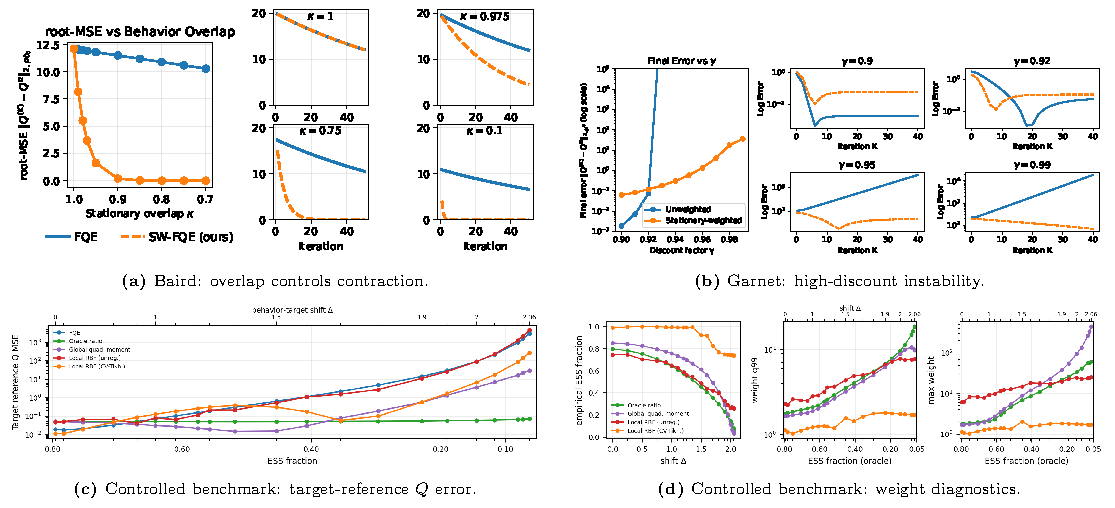
\includegraphics[width=\linewidth]{figures/experiments_composite.pdf}
 \caption{\textbf{A--B:} finite-state norm-mismatch examples. Stationary
weighting restores fast decay in Baird's example and prevents the high-discount
divergence seen in Garnet MDPs. \textbf{C--D:} continuous linear-Gaussian
simulation. Panel C plots target-stationary \(Q\)-error against the oracle
stationary-ratio effective sample size (ESS) fraction, with behavior--target
shift shown on the top axis. Stationary weighting reduces target-stationary
\(Q\)-error as overlap deteriorates. Panel D reports empirical ESS and
tail-weight diagnostics for oracle and estimated weights.}
    \label{fig:experiments-composite}
\end{figure}

The results illustrate the bias--variance tradeoff predicted by the theory.
Unweighted FQE is stable, but under behavior--target shift it fits the
misspecified affine \(Q\)-class in behavior-relevant regions, leading to larger
target-stationary error. Oracle weighting removes this projection mismatch and
gives the best attainable correction within the same \(Q\)-class. The
unregularized RBF moment estimator is unstable under limited coverage, producing
nonuniform weights that poorly approximate the oracle ratio. CV-Tikhonov
regularization gives a lower-variance correction and improves on unweighted FQE
under moderate-to-severe shift, but remains biased when overlap is poor. The
exponential-quadratic model performs best among estimated weights because its
log-ratio class is correctly specified in this benchmark, although its lower ESS
and larger maximum weights show the variance cost of ratio extrapolation.

We also compare against a closed-form minimax Bellman-residual estimator using
the same affine \(Q\)-class and an RBF critic. For both estimated weighting and
minimax fitting, Figure~\ref{fig:minimax-weighting-overlap} in
Appendix~\ref{app:minimax-baseline} reports deployable CV-tuned rules and
oracle-tuned diagnostics. The CV rules choose Tikhonov regularization by
held-out stationarity or Bellman moment risk, without using oracle
target-stationary error. Minimax fitting is competitive under favorable tuning,
but does not uniformly dominate stationary weighting in the deployable
finite-sample setting. This comparison suggests that stationary weighting is
best viewed as complementary to minimax Bellman-residual fitting: it preserves
the regression structure of FQE while targeting the norm in which policy
evaluation contracts.

\section{Conclusion}

We studied FQE without Bellman completeness through a norm-mismatch lens:
standard off-policy FQE projects Bellman targets in the behavior norm, whereas
policy evaluation contracts in the target stationary norm. Stationary-weighted
FQE changes only the regression weights, preserving FQE's supervised-learning
structure while aligning the fitted projection with this contraction. Our
finite-sample bound gives linear convergence to the stationary projected fixed
point under misspecification and off-policy sampling, separating
finite-iteration, statistical, Bellman approximation, and density-ratio
estimation errors. The result shows that Bellman completeness is not the only
way to control fitted iteration: one can instead align the projection norm with
the distribution under which policy evaluation is stable. The main limitations
are coverage and stable density-ratio estimation; Appendix~\ref{app:additional-conclusion}
discusses these limitations, connections to minimax Bellman methods, and future
directions.

 

\bibliographystyle{plainnat}
\bibliography{../../common/ref}

 
 
 

\appendix

\section{Expanded Conclusion}
 \label{app:additional-conclusion}

We studied FQE without Bellman completeness through a norm-mismatch lens:
standard off-policy FQE projects Bellman targets in the behavior norm, whereas
the target-policy Bellman operator contracts in the stationary norm.
Stationary-weighted FQE changes only the regression weights, preserving the
supervised-learning structure of FQE while aligning the projection norm with
this contraction. Our finite-sample bound gives linear convergence to the
stationary projected fixed point under misspecification and off-policy sampling,
separating finite-iteration, statistical, Bellman approximation, and
density-ratio estimation errors. The analysis further shows that approximate
density ratios affect FQE through curvature loss and a residual-interaction term
scaled by the inherent Bellman error.

The main practical limitations are coverage and density-ratio estimation. Poor
overlap can make exact stationary ratios unstable, suggesting a role for
discounted or regularized occupancy weights and stable balancing estimators in
limited-coverage regimes. Stationary weighting should therefore be viewed as
complementary to fitted Bellman-error minimization and minimax \(Q\)-learning
methods, rather than as a replacement. Minimax objectives provide a powerful way
to control Bellman residuals and can perform well with suitable tuning, while
stationary weighting offers a simple regression-based route for aligning the
fitted objective with the target-policy distribution. Because stationary ratios
enter through regression weights, approximate ratios can still be useful when
they move the fitted norm toward the target stationary distribution. In our
continuous benchmark, regularized estimated weights improve performance in
lower-overlap regimes and, when the correction is imperfect, remain close to
unweighted FQE.

Overall, stationary reweighting is a minimal modification of FQE that restores
the contraction geometry while making the usual coverage requirements explicit.
Understanding how stationary weighting and minimax objectives can be combined,
and how to tune them reliably under limited overlap, is an important direction
for future work.



\paragraph{Organization.} The appendix is organized as follows. Appendix~\ref{app:conditions} discusses
the regression-geometry condition and the residual interpolation bound, and
Appendix~\ref{app:approxwts} records consequences for approximate weights.
Appendix~\ref{app:implicit-stationary-sampling} treats implicit stationary
sampling with estimated rewards. Appendix~\ref{app:ratio-estimation} describes
stationary-ratio estimation, Appendix~\ref{sec::appendix} gives experimental
details, Appendix~\ref{appendix::stationary} collects contraction results, and
the final two sections prove the technical and main results.

\section{Additional Details}




\subsection{Algorithm}

\begin{algorithm}[h]
\caption{\textbf{Stationary-Weighted Fitted \(Q\)-Evaluation}}
\label{alg::sw-fqi}
\begin{algorithmic}[1]

\INPUT Offline data \(\mathcal D_n\), target policy \(\pi\),
function class \(\mathcal F\), iterations \(K\), discount \(\gamma\)

\ALGCOMMENT{Estimate stationary state-action density ratio}
\STATE \(\widehat w_\pi \gets\) estimator of \(w_\pi\)

\STATE Initialize \(\widehat Q^{(0)} \in \mathcal F\)

\FOR{\(k = 0,\dots,K-1\)}

  \ALGCOMMENT{Construct Bellman targets}
  \STATE \(Y_i^{(k)} \gets R_i + \gamma(\pi \widehat Q^{(k)})(S_i')\)

  \ALGCOMMENT{Stationary-weighted regression}
  \STATE \mbox{\(\widehat Q^{(k+1)} \gets
     \arg\min_{f \in \mathcal F}
     \sum_{i=1}^n \widehat w_\pi(S_i,A_i)
       \bigl\{Y_i^{(k)} - f(S_i,A_i)\bigr\}^2\)}

\ENDFOR

\OUTPUT \(\widehat Q^{(K)}\)

\end{algorithmic}
\end{algorithm}


\begin{figure}[t]
\centering
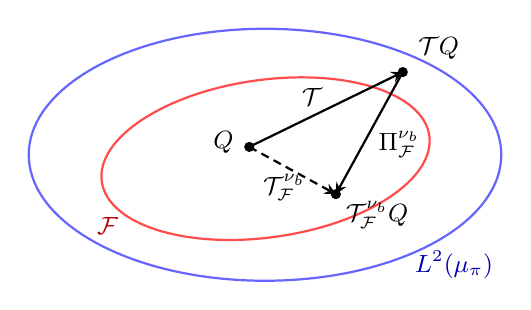
\begin{tikzpicture}[
    >=stealth,
    font=\small,
    every node/.style={inner sep=1pt}
]

% Blue: L2(mu) norm
\draw[thick, blue!60] (0,0) ellipse (3.0 and 1.6);
\node[blue!70!black] at (2.4,-1.4) {$L^2({\mu_\pi})$};

% Red: function class
\draw[thick, red!70, rotate=8] (0,-0.05) ellipse (2.1 and 1.0);
\node[red!70!black] at (-2,-0.9) {$\mathcal F$};

% Points
\coordinate (Q)   at (-0.2,0.1);
\coordinate (TQ)  at (1.75,1.05);
\coordinate (PTQ) at (0.9,-0.5);

\node[fill=black, circle, inner sep=1.3pt,
      label={[xshift=-3pt,yshift=-5pt]above left:{$Q$}}] at (Q) {};
\node[fill=black, circle, inner sep=1.3pt,
      label={[xshift=3pt,yshift=2pt]above right:{$\mathcal T Q$}}] at (TQ) {};
\node[fill=black, circle, inner sep=1.3pt,
      label={[xshift=1pt,yshift=-0pt]below right:{$\mathcal T_{\mathcal F}^{\nu_b}Q$}}] at (PTQ) {};

% Arrows
\draw[->, thick] (Q) -- (TQ)
    node[midway, above, xshift=-5pt] {$\mathcal T$};
\draw[->, thick] (TQ) -- (PTQ)
    node[midway, right, xshift=2pt, yshift=-4pt] {$\Pi_{\mathcal F}^{\nu_b}$};
\draw[->, thick, densely dashed] (Q) -- (PTQ)
    node[midway, below, xshift=-3pt] {$\mathcal T_{\mathcal F}^{\nu_b}$};

\end{tikzpicture}

\caption{Norm mismatch. The Bellman update \(\mathcal T Q\) may leave
\(\mathcal F\), so FQE projects it back using the behavior-distribution norm
\(L^2(\nu_b)\).
This projection need not preserve the contraction property of policy evaluation
in the stationary norm \(L^2(\mu_\pi)\).}
\label{fig::mismatch}
\end{figure}


\subsection{Extension to Admissible Weighting Functions}
\label{sec:admissible}

For clarity, the main text focuses on the stationary state-action density ratio
\(d\mu_\pi/d\nu_b\). The more general analysis separates two requirements. The
first is \emph{projection equivalence}: the reference weight must reproduce the
stationary projected Bellman update on \(\mathcal F\). This condition is weaker
than Bellman completeness. If \(\mathcal T(\mathcal F)\subseteq\mathcal F\), the
Bellman residual is zero, so the projection is exact and the choice of weights
is irrelevant.

\begin{enumerate}[label=\textbf{C\arabic*}, ref={C\arabic*}, leftmargin=1.5em,resume=cond]
\item \label{cond::overlap}
\textbf{Weighted projection equivalence.}
There exists a nonnegative \(w_{\pi}\in L^2(\nu_b)\) such that, for all
\(Q\in\mathcal F\),
\[
\Pi_{\mathcal F}\mathcal TQ
\in
\argmin_{f\in\mathcal F}
E_{\nu_b}\!\left[
w_{\pi}(S,A)\{\mathcal TQ(S,A)-f(S,A)\}^2
\right].
\]
\end{enumerate}

Condition~\ref{cond::overlap} says that the \(\mu_\pi\)-projected Bellman
update can also be obtained by weighted regression under the behavior
distribution. Exact stationary ratios are the canonical admissible weights when
\(\mu_\pi\ll\nu_b\), but other weights may also be admissible if they induce
the same projected Bellman update on \(\mathcal F\).

The second requirement is needed only to report errors in the stationary norm.

\begin{enumerate}[label=\textbf{C\arabic*}, ref={C\arabic*}, leftmargin=1.5em,resume=cond]
\item \label{cond::norm-compare}
\textbf{Weighted--stationary norm comparison.}
There exists \(1\le c<\infty\) such that, for all \(f\in L^2(\mu_\pi)\),
\[
c^{-1}\|f\|_{2,\mu_\pi}
\le
\|f\|_{2,w_\pi\nu_b}
\le
c\|f\|_{2,\mu_\pi}.
\]
\end{enumerate}

For the stationary density ratio, \(w_\pi\nu_b=\mu_\pi\), so
Condition~\ref{cond::overlap} holds by identity of the two projection problems
and Condition~\ref{cond::norm-compare} holds with \(c=1\).

Hereafter, \(\widehat w_\pi\) denotes an estimator of a weight \(w_\pi\)
satisfying Condition~\ref{cond::overlap}. The stationary state-action density
ratio is the canonical choice, but the analysis applies to any admissible
weighting function.

\textbf{Relation to minimax \(Q\)-learning.}
Condition~\ref{cond::overlap} is related to dual realizability assumptions in
minimax and saddle-point approaches
\citep{uehara2020minimax,xie2021bellman,imaizumi2021minimax,
uehara2023offline,zanette2022bellman}. Both require coverage of a target
state-action distribution. Minimax methods typically use the discounted
occupancy measure and require the relevant ratio or moment equation to be
represented by an auxiliary critic class
\citep[see, e.g., Section~6 of][]{xie2021bellman}. We instead treat the weights
as an estimated input to fitted regression and quantify how approximate
admissible weighting affects the FQE recursion.


\subsection{Discussion of Regression-Geometry Conditions}
\label{app:conditions}

Condition~\ref{cond::weight-stability} is a localized curvature condition for
the fitted regression problem. It requires the estimated weighted norm to be a
relative perturbation of the ideal weighted norm on
\(\mathcal H_{\mathcal F}:=\mathcal F-\mathcal F\). A simple sufficient
condition is
\[
\left\|\frac{\widehat w_\pi}{w_\pi}-1\right\|_\infty<1,
\]
which implies
\[
\rho_{\mathcal H}
\le
\left\|\frac{\widehat w_\pi}{w_\pi}-1\right\|_\infty < 1 .
\]

For finite-dimensional linear classes, this condition reduces to a Gram-matrix
condition. If
\(\mathcal H_{\mathcal F}\subseteq\{x\mapsto \phi(x)^\top u:u\in\mathbb R^p\}\),
define
\[
G
:=
E_{\nu_b}\!\left[w_\pi(X)\phi(X)\phi(X)^\top\right],
\qquad
\Delta_G
:=
E_{\nu_b}\!\left[
\{\widehat w_\pi(X)-w_\pi(X)\}\phi(X)\phi(X)^\top
\right].
\]
Then Condition~\ref{cond::weight-stability} holds if
\[
\rho_G
:=
\left\|
G^{-1/2}\Delta_GG^{-1/2}
\right\|_{\mathrm{op}}
<1,
\]
where the inverse is taken on the support of \(G\). In this case,
\(\rho_{\mathcal H}\le \rho_G\), and
\(\widehat G:=G+\Delta_G\) satisfies
\[
(1-\rho_G)u^\top Gu
\le
u^\top \widehat G u
\le
(1+\rho_G)u^\top Gu
\qquad\text{for all }u .
\]



\begin{remark}[Localized curvature]
\label{rem:localized-curvature}
The global curvature condition in Condition~\ref{cond::weight-stability} can be
weakened to a localized version. For \(r>0\), define
\[
\rho_{\mathcal H}(r)
:=
\sup_{\substack{h\in\mathcal H_{\mathcal F}\\
\|h\|_{2,w_\pi\nu_b}\ge r}}
\left|
\frac{E_{\nu_b}[(\widehat w_\pi-w_\pi)h^2]}
     {E_{\nu_b}[w_\pi h^2]}
\right|.
\]
If \(\rho_{\mathcal H}(r)<1\), the proof of
Lemma~\ref{lemma::errorperiter2} yields the one-step bound
\[
\|\mathcal T_{\mathcal F}(\hat Q^{\mathrm{init}})-\hat Q_n\|_{2,w_\pi\nu_b}
\le
\max\left\{
r,\,
\frac{C}{1-\rho_{\mathcal H}(r)}
\left[
\kappa_{\mathrm{cov}}\left(\delta_n+\sqrt{\frac{\log(1/\tau)}{n}}\right)
+\omega_{\mathrm{Bell},w}
\right]
\right\}.
\]
Indeed, if the fitted error direction has weighted norm below \(r\), the bound
is immediate; otherwise, the same quadratic-curvature argument applies with
\(\rho_{\mathcal H}(r)\) in place of \(\rho_{\mathcal H}\).

The useful choice is to take \(r\) at the one-step error scale. Writing
\[
a_n
:=
\kappa_{\mathrm{cov}}\left(\delta_n+\sqrt{\frac{\log(1/\tau)}{n}}\right)
+\omega_{\mathrm{Bell},w},
\]
one may choose \(r\asymp a_n\), or more generally the smallest radius for which
\(\rho_{\mathcal H}(r)\le\rho_0<1\). Then the localized bound gives
\[
\|\mathcal T_{\mathcal F}(\hat Q^{\mathrm{init}})-\hat Q_n\|_{2,w_\pi\nu_b}
\lesssim a_n .
\]
Thus curvature is only needed above the statistical error scale: if the fitted
error is smaller than \(r\), the desired bound already holds, while larger
directions are controlled by the localized curvature condition.

A sufficient localized condition is
\[
B_{\mathcal H}(r)
\left\|\frac{\widehat w_\pi}{w_\pi}-1\right\|_{2,w_\pi\nu_b}<1,
\qquad
B_{\mathcal H}(r)
:=
\sup_{\substack{h\in\mathcal H_{\mathcal F}\\
\|h\|_{2,w_\pi\nu_b}\ge r}}
\frac{\|h\|_{4,w_\pi\nu_b}^2}{\|h\|_{2,w_\pi\nu_b}^2}.
\]
This localized form is useful for rich classes in which the global
\(L^4\)-to-\(L^2\) comparison may fail because of highly concentrated
directions, while curvature above the statistical error scale remains
controlled.
\end{remark}


\begin{remark}[Approximate Bellman completeness ]
Approximate Bellman completeness enters through
\(\omega_{\mathrm{Bell},w}\). A simple sup-norm bound is
\[
\omega_{\mathrm{Bell},w}
\le
c\left\|\frac{\widehat w_\pi}{w_\pi}-1\right\|_\infty
\varepsilon_{\mathrm{Bell}},
\]
with the same extended-ratio convention on \(\{w_\pi=0\}\). More generally, if
\[
\|\mathcal TQ-\mathcal T_{\mathcal F}Q\|_\infty
\le
L_{\mathcal R}
\|\mathcal TQ-\mathcal T_{\mathcal F}Q\|_{2,\mu_\pi}^{\beta}
\qquad\text{for all }Q\in\mathcal F,
\]
then
\[
\omega_{\mathrm{Bell},w}
\le
L_{\mathcal R}\varepsilon_w\varepsilon_{\mathrm{Bell}}^\beta .
\]

This residual interpolation condition holds with \(\beta=0\) under uniform
boundedness of the Bellman residual class. Larger exponents are available when
the residual class
\(\{\mathcal TQ-\mathcal T_{\mathcal F}Q:Q\in\mathcal F\}\) is smoother or
lower-dimensional. For a finite-dimensional linear residual class with a
nondegenerate Gram matrix and bounded features, norm equivalence gives
\(\beta=1\). For a \(d\)-variate Hölder ball of smoothness \(s>0\), the standard
Hölder interpolation inequality gives
\[
\|r\|_\infty
\le
C\|r\|_{2,\mu_\pi}^{2s/(2s+d)},
\]
so \(\beta=2s/(2s+d)\). For Sobolev or RKHS balls of smoothness \(s>d/2\), the
Gagliardo--Nirenberg/Sobolev interpolation inequality gives
\[
\|r\|_\infty
\le
C\|r\|_{2,\mu_\pi}^{1-d/(2s)},
\]
so \(\beta=1-d/(2s)\). For signed convex hulls of uniformly bounded
dictionaries, one generally obtains only the bounded-class case \(\beta=0\). If
the hull is restricted to an \(m\)-dimensional or \(s_0\)-sparse subspace with a
nondegenerate Gram matrix, the finite-dimensional norm-equivalence case gives
\(\beta=1\), with constants depending on \(m\) or \(s_0\). These are standard
interpolation and entropy consequences for RKHS balls, signed convex hulls, and
Hölder or Sobolev classes
\citep{mendelson2010regularization,van2014uniform,bibaut2021sequential,
adams2003sobolev,triebel2006theory}. 
\end{remark}




\subsection{Discussion of Main Result}
\label{app:approxwts}
\paragraph{Contraction under approximate stationary density-ratio weights.}
The analysis extends beyond exact recovery of \(w_\pi\). Suppose
\(\overline w_\pi\) is a limiting weight and the projected Bellman operator is
contractive in \(L^2(\overline w_\pi\nu_b)\) with factor
\(\overline\gamma<1\). Then the same inexact Picard argument applies with
\(\overline\gamma\) in place of \(\gamma\), and with the corresponding projected
fixed point under the \(\overline w_\pi\nu_b\)-weighted norm. Thus, even
misspecified weights can improve stability if they move the projection norm
closer to one in which the Bellman operator is contractive.

A simple sufficient condition is multiplicative closeness to the stationary
ratio:
\[
(1-\varepsilon)w_\pi(s,a)
\le
\overline w_\pi(s,a)
\le
(1+\varepsilon)w_\pi(s,a).
\]
Then \(L^2(\overline w_\pi\nu_b)\) and \(L^2(w_\pi\nu_b)=L^2(\mu_\pi)\) are
equivalent. In particular,
\[
\|f\|_{2,\mu_\pi}^2
\le
\frac{1}{1-\varepsilon}\|f\|_{2,\overline w_\pi\nu_b}^2,
\qquad
\|f\|_{2,\overline w_\pi\nu_b}^2
\le
(1+\varepsilon)\|f\|_{2,\mu_\pi}^2 .
\]
Since \(\mathcal T\) is a \(\gamma\)-contraction in \(L^2(\mu_\pi)\), it is a
\[
\overline\gamma
\le
\gamma\sqrt{\frac{1+\varepsilon}{1-\varepsilon}}
\]
contraction in \(L^2(\overline w_\pi\nu_b)\), provided the right-hand side is
less than one. Thus small multiplicative weight errors preserve contraction up
to an inflated contraction factor.

\paragraph{On-policy and ergodic limits.}
When \(\nu_b=\mu_\pi\), the stationary state-action density ratio is
\(w_\pi\equiv1\), so stationary-weighted FQE reduces to ordinary FQE and the
weight-related terms vanish. More generally, under ergodic on-policy trajectory
sampling, empirical state-action visitation frequencies converge to
\(\mu_\pi\). Thus the empirical regression norm approaches the stationary norm,
and ordinary FQE inherits the same contraction property asymptotically, up to
sampling error.

\subsection{Implicit Stationary Weighting by Sampling}
\label{app:implicit-stationary-sampling}

Stationary weighting can also be achieved implicitly when the transition kernel
\(P\), and hence \(\mu_\pi\), is known. If we can sample
\((\widetilde S_i,\widetilde A_i,\widetilde S_i')\sim \mu_\pi\otimes P\)
directly, then the regression design is already matched to the target
stationary distribution. The only missing quantity is the reward, which must be
estimated from the behavior data. Let \(\widehat r\) denote such an estimate,
and run unweighted FQE on
\[
\{(\widetilde S_i,\widetilde A_i,
\widehat r(\widetilde S_i,\widetilde A_i),\widetilde S_i')\}_{i=1}^n .
\]
This is ordinary stationary-sampling FQE with \(w_\pi\equiv 1\), but with a
perturbed reward.

Define
\[
\widehat{\mathcal T}Q:=\widehat r+\gamma P_\pi Q,
\qquad
\widehat{\mathcal T}_{\mathcal F}:=\Pi_{\mathcal F}\widehat{\mathcal T},
\]
and let \(\widehat Q^\pi_{\mathcal F}\) be the fixed point of
\(\widehat{\mathcal T}_{\mathcal F}\). For the \(K\)-step iterate
\(\widehat Q^{(K)}\),
\[
\|\widehat Q^{(K)}-Q^\pi_{\mathcal F}\|_{2,\mu_\pi}
\le
\|\widehat Q^{(K)}-\widehat Q^\pi_{\mathcal F}\|_{2,\mu_\pi}
+
\|\widehat Q^\pi_{\mathcal F}-Q^\pi_{\mathcal F}\|_{2,\mu_\pi}.
\]
The first term is the usual finite-iteration and statistical error under
stationary sampling. The second term is the reward-estimation perturbation.

\begin{theorem}[Reward perturbation]
\label{theorem:reward-perturbation}
Under Conditions~\ref{cond::stationary}--\ref{cond::convex},
\[
\|\widehat Q^\pi_{\mathcal F}-Q^\pi_{\mathcal F}\|_{2,\mu_\pi}
\le
\frac{1}{1-\gamma}
\|\widehat r-r_0\|_{2,\mu_\pi}.
\]
If, in addition, \(\mathcal F\) is a linear subspace of \(L^2(\mu_\pi)\), then
\[
\|\widehat Q^\pi_{\mathcal F}-Q^\pi_{\mathcal F}\|_{2,\mu_\pi}
\le
\frac{1}{1-\gamma}
\|\Pi_{\mathcal F}(\widehat r-r_0)\|_{2,\mu_\pi}.
\]
\end{theorem}


 
 




\section{Details on Stationary-Ratio Estimation}
\label{app:ratio-estimation}

Stationary-weighted FQE requires weights approximating the stationary
state-action density ratio \(w_\pi=d\mu_\pi/d\nu_b\). Estimating such ratios is a well-studied
problem, often formulated through DICE-style saddle-point objectives
\citep{nachum2019dualdice,zhang2020gendice,lee2021optidice} or related
balancing-weight methods \citep{uehara2020minimax,wang2023projected}.
Stationary ratios are the undiscounted analogues of discounted occupancy ratios
and can be obtained as a \(\gamma\to1\) limit under suitable normalization and
standard ergodicity conditions.

The key identifying condition is stationarity. Since \(w_\pi\nu_b=\mu_\pi\) is
stationary for \((\pi,P)\), the ratio satisfies
\begin{equation}
\label{eqn:app-stationary-moment}
E\!\left[
w_\pi(S,A)\{g(S,A)-g(S',A')\}
\right]=0
\qquad \text{for all } g,
\end{equation}
where \((S,A)\sim\nu_b\), \(S'\sim P(\cdot\mid S,A)\), and
\(A'\sim\pi(\cdot\mid S')\). Conversely, if a nonnegative function \(w\)
satisfies \eqref{eqn:app-stationary-moment} for all bounded measurable \(g\)
and \(E_{\nu_b}w(S,A)=1\), then \(w\nu_b\) is a stationary state-action
distribution for \((\pi,P)\). Thus, when the stationary distribution is unique,
\(w=w_\pi\) \(\nu_b\)-almost surely.

Minimax and DICE-style estimators enforce \eqref{eqn:app-stationary-moment}
over a critic class \(\mathcal G\) while searching over a ratio class
\(\mathcal W\). A representative empirical estimator is
\begin{equation}
\label{eqn:app-ratio-objective}
\begin{aligned}
\widehat w_\pi
&\in
\arg\min_{w\in\mathcal W}
\Biggl[
\sup_{g\in\mathcal G}
\left\{
\frac{1}{n}\sum_{i=1}^n
w(S_i,A_i)\{g(S_i,A_i)-g(S_i',A_i')\}
-
\frac{1}{2n}\sum_{i=1}^n g(S_i,A_i)^2
\right\}
\\
&\qquad\qquad+
\left(
\frac{1}{n}\sum_{i=1}^n w(S_i,A_i)-1
\right)^2
\Biggr],
\end{aligned}
\end{equation}
where \(A_i'\sim\pi(\cdot\mid S_i')\). The final term enforces normalization.
The quadratic term in \(g\) makes the inner problem strongly concave and turns
the supremum into a squared measure of stationarity-moment violation. Other
DICE variants use different convex regularizers, discounted-moment constraints,
or additional normalization and positivity penalties, but they share the same
stationarity-moment structure.

When \(\mathcal G\) is linear or an RKHS, the inner maximization in
\eqref{eqn:app-ratio-objective} often has a closed form. For example, suppose
\(g_\theta(x)=\theta^\top\phi(x)\), where \(x=(s,a)\). For a fixed candidate
ratio \(w\), define
\[
\widehat m_w
:=
\frac{1}{n}\sum_{i=1}^n
w(S_i,A_i)\{\phi(S_i,A_i)-\phi(S_i',A_i')\},
\qquad
\widehat\Sigma
:=
\frac{1}{n}\sum_{i=1}^n
\phi(S_i,A_i)\phi(S_i,A_i)^\top .
\]
Adding ridge regularization \(\lambda\|\theta\|_2^2/2\), the inner supremum is
\[
\sup_\theta
\left\{
\theta^\top \widehat m_w
-
\frac{1}{2}\theta^\top(\widehat\Sigma+\lambda I)\theta
\right\}
=
\frac{1}{2}\widehat m_w^\top
(\widehat\Sigma+\lambda I)^{-1}
\widehat m_w .
\]
Thus the ratio estimator can be viewed as choosing \(w\) to balance stationary
flow moments in the feature space \(\phi\). RKHS critics give an analogous
kernelized discrepancy between the weighted current state-action distribution
and the induced next state-action distribution. These structured critic classes
can yield stable, computationally simple weights while still approximating the
stationary projection norm
\citep{dikkala2020minimax,uehara2020minimax,wang2023projected,
olivas2025source}.

For numerical stability, practical implementations often regularize or truncate
the estimated ratio, for example using Tikhonov regularization
\citep{uehara2021finite}. Common choices include constraining \(w\ge 0\), adding
an \(\ell_2\) or entropy penalty on \(w\), clipping large weights, or estimating
a discounted occupancy ratio with discount close to one. Such regularization
trades small bias for lower variance and better conditioning, which is often
important under limited overlap.
 

\paragraph{Instantiating relative weight error.}
The generic term
\(\|\widehat w_\pi/w_\pi-1\|_{2,w_\pi\nu_b}\) is useful for sufficient bounds on
the residual interaction and can be controlled using guarantees for specific
minimax or saddle-point ratio estimators. Analyses for conditional
moment problems are given by
\citet{dikkala2020minimax,olivas2025source}, and off-policy weighting analyses
are given by \citet{uehara2020minimax,wang2023projected}. At a high level, such
bounds decompose into weight-class approximation, critic-class approximation,
and statistical error:
\[
\inf_{w\in\mathcal W}\|w-w^\dagger\|
+
\inf_{g\in\mathcal G}\|g-g^\dagger\|
+
\mathrm{stat}(\mathcal W,\mathcal G,n),
\]
where \(\mathcal W\) and \(\mathcal G\) are the ratio and critic classes, and
\(\mathrm{stat}(\mathcal W,\mathcal G,n)\) is controlled by localized
complexity; see also \citet{bennett2023minimax}.


\subsection{Fixed-Point Estimation of Stationary Ratios}
\label{sec::fixedstationary}

The stationary state-action density ratio
$w_{\pi} = d{\mu_\pi} / d\nu_b$ is identified by the fixed-point equation
implied by stationarity ${\mu_\pi} = {\mu_\pi} P_\pi$:
\[
w_{\pi}(s',a') = (\mathcal K w_{\pi})(s',a'),
\]
where the linear operator $\mathcal K$ is
\[
(\mathcal K g)(s',a')
=
\frac{\pi(a' \mid s')}{\nu_b(a' \mid s')}
\,\E_{(S,A)\sim\nu_b}\!\left[g(S,A)\,k(S,A,s')\right],
\]
and
\[
k(s,a,s')
=
\frac{P(s' \mid s,a)}{\rho_{b,1}(s')},
\qquad
\rho_{b,1}(s')
:=
\E_{(S,A)\sim\nu_b}\!\left[P(s' \mid S,A)\right].
\]
Here \(k\) is the transition density ratio and \(\rho_{b,1}\) is the marginal
density of \(S'\) induced by the behavior dynamics.
The quantity $k$ can be estimated directly using the empirical squared-loss
objective of \citet{hines2025learning}:
\[
\frac{1}{n^2}\sum_{i=1}^n \sum_{j=1}^n
k(S_i,A_i,S_j')^2
\;-\;
\frac{2}{n}\sum_{i=1}^n k(S_i,A_i,S_i').
\]

However, $\mathcal K$ is the adjoint of $P_\pi$ in $L^2({\mu_\pi})$ and satisfies
$\|\mathcal K\|_{L^2({\mu_\pi})} = 1$, so direct Picard iteration of 
$w_{\pi} = \mathcal K w_{\pi}$ is not contractive. A standard workaround is the
discounted resolvent equation
\[
d_{\gamma'} = (1-\gamma')\tfrac{\pi}{\nu_b} + \gamma'\,\mathcal K d_{\gamma'},
\]
whose solution $d_{\gamma'}$ is the $\gamma'$-discounted occupancy ratio.
The resolvent replaces exact stationarity by a $\gamma'$-discounted moment
balance, which yields a $\gamma'$-contractive update. Since $\mathcal K$ is
nonexpansive in $L^2({\mu_\pi})$, Picard iteration applies and 
\(d_{\gamma'}\) can be computed analogously to fitted value iteration.

Under standard ergodicity assumptions---irreducibility, aperiodicity, and geometric
mixing---the discounted ratios satisfy \(d_{\gamma'} \to w_{\pi}\) as \(\gamma' \uparrow 1\)
\citep{meyn1993markov, glynn1996liapounov}. The resolvent formulation induces a
familiar bias--variance trade-off: larger \(1-\gamma'\) improves numerical
stability but introduces bias of order $O(1-\gamma')$, whereas letting
$\gamma' \uparrow 1$ removes the bias at the expense of variance scaling like
$(1-\gamma')^{-1}$ due to the effective horizon of the discounted occupancy
measure.




 

 

\section{Experiments}
\label{sec::appendix}

\subsection{Finite-State Diagnostic Experiments}
\label{app:toy_norm_mismatch}

\paragraph{Baird hub-and-spokes.}
The Baird experiment uses a hub state and six spoke states
\citep{baird1995residual}. The solid action moves deterministically to the hub;
the dashed action moves uniformly to one of the spokes. The target policy always
takes the solid action. The behavior policy takes the solid action with
probability \(\kappa\), so decreasing \(\kappa\) reduces stationary overlap with
the target policy. We use the standard seven-dimensional linear feature map,
zero rewards, ridge-regularized least squares at each FQE step, and exact
stationary ratios. Since \(Q^\pi\equiv0\), the experiment isolates whether the
projected Bellman iteration contracts in the intended norm. Reported curves are
averaged over 100 independent datasets.

\paragraph{Sparse Garnet MDPs.}
The Garnet experiment uses random MDPs with \(100\) states, \(4\) actions, and
branching factor \(5\). For each state-action pair, five next states are sampled
without replacement and assigned Dirichlet transition probabilities. Rewards
are Gaussian. The target policy is sampled randomly; the behavior policy is
\(\varepsilon\)-greedy with \(\varepsilon=0.1\). Data are generated with a reset
scheme that deliberately breaks stationarity. The linear feature class has
dimension \(5\) and contains \(Q^\pi\), but is generically not Bellman complete.
Thus any instability is due to the fitted projection geometry, not ordinary
realizability failure. The main figure uses exact stationary ratios; the same
qualitative stabilization was also observed with tabular DualDICE-style ratio
estimates.

\subsection{Controlled linear-Gaussian simulation}

The continuous benchmark uses \(S_t\in\mathbb R^2\) and \(A_t\in\mathbb R\).
The dynamics are linear Gaussian,
\[
S_{t+1}=B S_t + C A_t+\epsilon_t,
\qquad
\epsilon_t\sim N(0,\sigma^2 I),
\]
with quadratic reward
\[
r(s,a)=-\|s-s^\star\|^2-\lambda a^2 .
\]
The target and behavior policies are Gaussian linear policies,
\[
A_t^\pi\mid S_t=s \sim N(K_\pi s,\sigma_\pi^2),
\qquad
A_t^b\mid S_t=s \sim N(K_b s,\sigma_b^2),
\]
where \(K_b=K_\pi+\Delta v\). The scalar \(\Delta\) controls the
behavior--target shift. We evaluate 100 independent replications over
\[
\begin{aligned}
\Delta\in\{&
0,0.25,0.5,0.75,0.9,1.0,1.1,1.2,1.25,1.35,\\
&1.5,1.6,1.7,1.8,1.9,1.95,2.0,2.025,2.05,2.055,2.06\}.
\end{aligned}
\]
The shift direction is scaled so that the closed-loop behavior process remains
stable throughout the sweep. The target action standard deviation is \(0.10\),
the behavior action standard deviation is \(0.15\), and the process-noise
standard deviation is \(0.12\). Thus \(\Delta=0\) gives high overlap, but is not
exactly on-policy because the behavior and target policies have different
action variances.

Because the system is linear Gaussian with quadratic rewards, \(Q^\pi\),
\(V^\pi\), and the discounted policy value \(\psi_\pi\) are computed
analytically by a quadratic fixed-point recursion. For the main stationary
weighting experiments, the reference distribution is the stationary Gaussian
state-action distribution under the target policy, and oracle weights are
stationary Gaussian density ratios. Discounted occupancy variants are evaluated
using Gaussian-mixture representations over time.

Offline data are sampled from the behavior stationary distribution. The value
discount in the Bellman targets is \(\gamma=0.95\). The regression weights
target the stationary state-action ratio \(d\mu_\pi/d\nu_b\), where
\(\mu_\pi\) is the target stationary state-action distribution and \(\nu_b\) is
the behavior sampling distribution.

We use the deliberately misspecified affine class \([1,s_1,s_2,a]\). Linear FQE
uses analytic target-action expectations, so the Bellman targets do not include
Monte Carlo integration error.

The ratio estimator is the finite-dimensional closed-form version of the
stationarity minimax moment problem, with a mean-one normalization. Let
\(z=(s,a)\). The ratio features \(\phi_w(z)\) consist of
\((1,z_1,z_2,z_3,z_1^2,z_2^2,z_3^2)\) and 64 Gaussian RBF features on \(z\);
the centers are evenly spaced behavior-sample points and the bandwidth is the
median center distance. Define
\[
\Delta_\pi\phi_w(s,a,s')
  =
  \phi_w(s,a)-\gamma_{\rm ratio}
    E_{a'\sim\pi(\cdot\mid s')}\{\phi_w(s',a')\},
\qquad
m_0=E_{s_0,a_0\sim\pi}\{\phi_w(s_0,a_0)\}.
\]
For \(w_\alpha(z)=\phi_w(z)^\top\alpha\), the reduced minimax estimator solves
\[
\min_\alpha
\left\|
\mathbb P_n w_\alpha(Z)\Delta_\pi\phi_w
-(1-\gamma_{\rm ratio})m_0
\right\|^2_{(B_n+\lambda_d I)^{-1}}
\;+\;\lambda_p\|\alpha\|_2^2
\;+\;\lambda_0\{\mathbb P_n w_\alpha(Z)-1\}^2,
\]
where \(B_n=\mathbb P_n\phi_w(Z)\phi_w(Z)^\top\), \(\lambda_0=10\), and
\(\gamma_{\rm ratio}=1\) unless otherwise stated. In the stationary case, the
flow right-hand side is zero and the mean-one penalty fixes the scale. Negative
fitted weights are floored at \(10^{-8}\), and all weights are normalized to
have empirical mean one before fitting FQE.

We use 64 standardized RBF ratio features and also include a positive
exponential-quadratic moment model
\[
w_\theta(s,a)=\exp\{\theta^\top\psi(s,a)\},
\]
where \(\psi\) contains standardized quadratic state-action features. Both
estimated ratio classes are fit only from stationarity moments. For stability,
we consider several additional regularization and truncation choices. Fixed
truncation uses \(\bar w_i\propto\min\{w_i,2\}\). ESS-adaptive winsorization
chooses the largest empirical cap \(c\) such that
\[
  \mathrm{ESS}(\bar w)/n
  =
  \frac{(\sum_i\bar w_i)^2}{n\sum_i\bar w_i^2}
  \ge0.60 .
\]
CV truncation chooses \(c\in\{1.5,2,3,5,10,25,\infty\}\) by three-fold
held-out stationarity risk, evaluating the ratio objective on held-out
\((S,A,S')\) after fitting \(\alpha\) on the other folds. CV-Tikhonov chooses
\(\lambda_p=\lambda_d\) from
\[
\{10^{-5},3{\cdot}10^{-5},10^{-4},3{\cdot}10^{-4},\ldots,3,10\}
\]
by five-fold held-out ratio risk and then refits on all offline data. These
selection criteria use only transition tuples \((S,A,S')\), not rewards or
oracle evaluation targets.

The primary metric is mean squared \(Q\)-error under the target stationary
distribution. Effective sample size, upper weight quantiles, and maximum
weights are reported as overlap diagnostics as the behavior policy moves away
from the target policy.

We also include a direct minimax Bellman-residual baseline. With
\(Q_\theta(s,a)=\phi_Q(s,a)^\top\theta\) and critic features \(\psi(s,a)\), this
baseline solves
\[
\min_\theta
\left\|
\mathbb P_n\psi(S,A)
\{Q_\theta(S,A)-R-\gamma E_\pi Q_\theta(S',A')\}
\right\|_{(\mathbb P_n\psi\psi^\top+\lambda_d I)^{-1}}^2
\;+\;\lambda_q\|\theta\|_2^2 .
\]
The main comparison uses the same affine \(Q\)-class as FQE and the same RBF
critic features used for ratio fitting. The practical minimax row chooses a
dimensionless Tikhonov level \(\eta\) by held-out Bellman moment risk, using
\[
\lambda_d=\eta\,\mathrm{tr}(\mathbb P_n\psi\psi^\top)/d_\psi
\]
and the analogous normalized ridge for the reduced \(Q\)-system. This baseline
is not a weighted FQE estimator; it is included to compare stationary weighting
with a standard Bellman-moment stabilization. For local RBF weighting,
correctly specified quadratic weighting, and minimax fitting, we also report
oracle-tuned diagnostics that select the regularization level by
target-stationary \(Q\)-error on an independent evaluation sample. These
oracle-tuned rows are diagnostic and are not used as deployable tuning rules.


\subsection{Practical and oracle-tuned Bellman baseline comparison}
\label{app:minimax-baseline}

Figure~\ref{fig:minimax-weighting-overlap} compares deployable and oracle-tuned
versions of the stationary-weighted and minimax Bellman baselines. The results
show that minimax Bellman methods can perform very well when tuned to oracle
target-stationary error, consistent with their theoretical motivation, but also
illustrate a common practical challenge for minimax approaches: deployable
tuning by held-out moment risk can be difficult and need not select the
configuration with the best target-stationary \(Q\)-error.

\begin{figure}[htb]
    \centering
    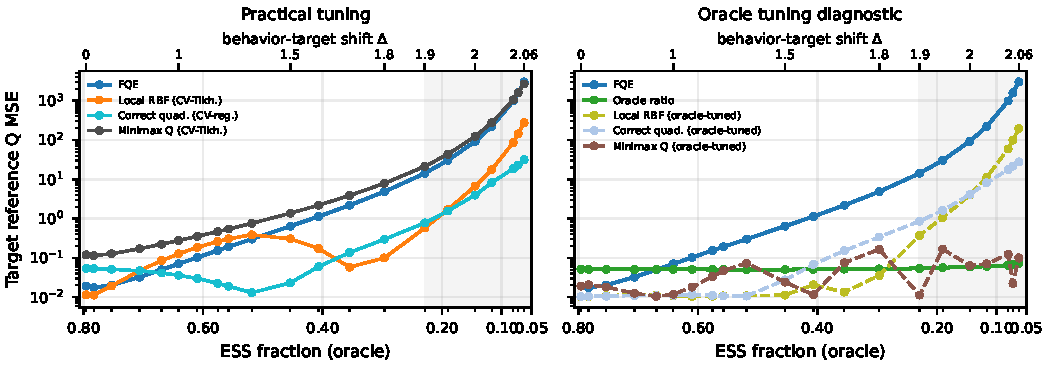
\includegraphics[width=\linewidth]{figures/oracle_practical_tuned_comparison.pdf}
    \caption{\textbf{Practical and oracle-tuned Bellman baselines.} Both panels
    plot target-stationary \(Q\)-error versus oracle ESS fraction, with
    behavior--target shift shown on the top axis. Left: deployable tuning rules
    based on held-out moment risks. Right: oracle-tuned diagnostics that select
    ridge parameters using independent target-stationary error. Practical
    stationary weighting improves over unweighted FQE in lower-overlap regimes,
    while oracle-tuned weighting and minimax rows show the attainable
    performance of the corresponding estimator classes.}
    \label{fig:minimax-weighting-overlap}
\end{figure}

\begin{figure}[t]
    \centering
    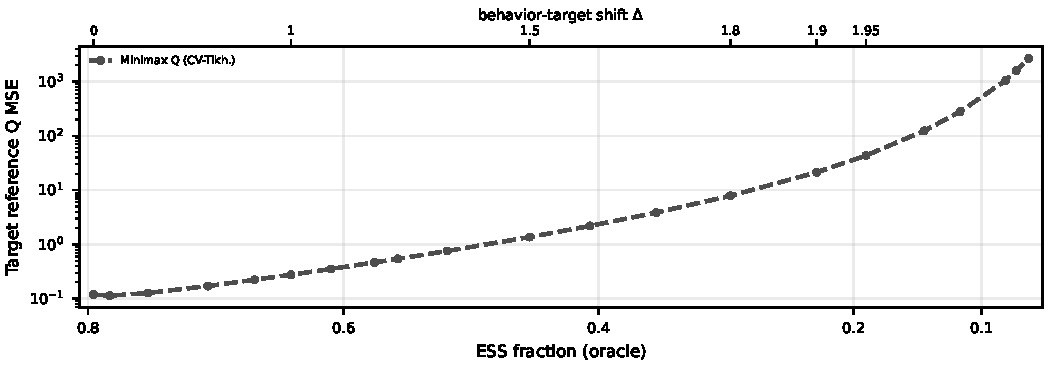
\includegraphics[width=\linewidth]{figures/minimax_tuning_sensitivity.pdf}
    \caption{\textbf{Minimax regularization sensitivity.} The minimax Bellman
    baseline is sensitive to the normalized Tikhonov level: weak regularization
    is high variance, while overly large ridges bias the Bellman moment fit.
    The CV-Tikhonov row selects the ridge by held-out Bellman moment risk.}
    \label{fig:minimax-tuning-sensitivity}
\end{figure}

As a diagnostic control, we also ran a flexible outer \(Q\)-class using the same
standardized RBF feature map as the ratio critic. In this setting, standard FQE
is already accurate under good overlap, while minimax fitting is stable but more
biased; under the most severe shifts, minimax remains finite when ordinary FQE
extrapolates poorly. This check confirms that the main linear-Gaussian
benchmark is not driven by a degenerate simulator, but it is not used as the
primary comparison.

\begin{figure}[t]
    \centering
    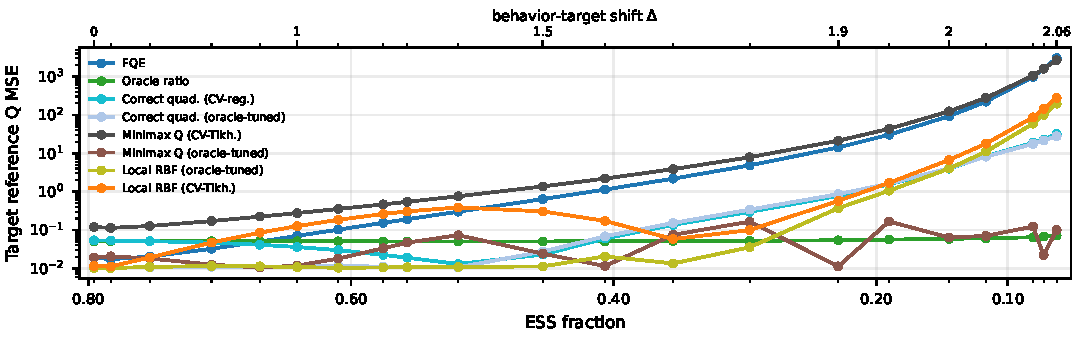
\includegraphics[width=\linewidth]{figures/gamma_sweep_stabilization_comparison_q_mse.pdf}
    \caption{\textbf{Stabilization comparison in the controlled
    linear-Gaussian benchmark.} Standard FQE is fit in the behavior norm.
    Oracle stationary weighting shows the target-stationary projection mechanism.
    The estimated-weight rows compare unregularized weights, a prespecified cap,
    ESS-adaptive winsorization, CV-Tikhonov ratio regularization, and CV
    truncation. The CV criteria use
    held-out stationarity moment risk and do not use rewards or oracle
    evaluation targets.}
    \label{fig:linear-gaussian-stabilization}
\end{figure}

\begin{figure}[t]
    \centering
    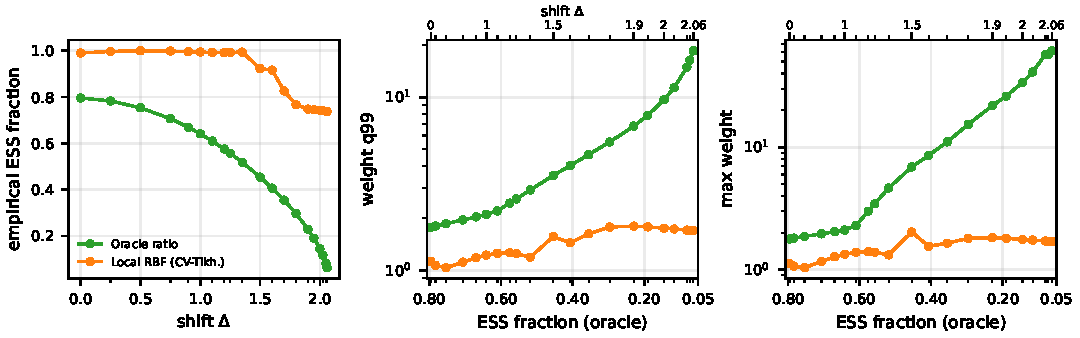
\includegraphics[width=\linewidth]{figures/gamma_sweep_weight_quality_all_stabilizers.pdf}
    \caption{\textbf{Weight diagnostics for all stabilizers in the controlled
    linear-Gaussian benchmark.} The main text reports only the oracle,
    unregularized, and CV-Tikhonov weights. Here we also show the prespecified
    cap, ESS-adaptive winsorization, and CV-truncated cap used in the stabilizer
    comparison.}
    \label{fig:linear-gaussian-weight-diagnostics-all}
\end{figure}

\begin{figure}[t]
    \centering
    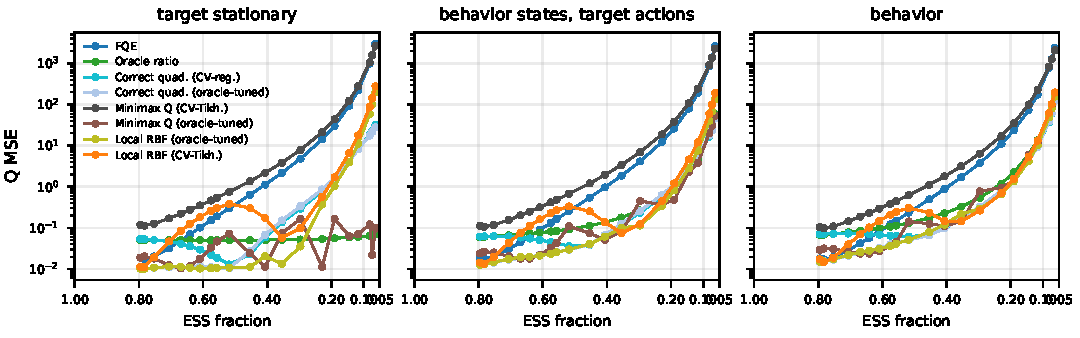
\includegraphics[width=\linewidth]{figures/gamma_sweep_norm_diagnostic_q_mse.pdf}
    \caption{\textbf{Norm diagnostics for the controlled linear-Gaussian
    benchmark.} Target-stationary error is the policy-evaluation norm used in
    the main panel. The behavior-state/target-action and behavior-norm panels
    show that the gains are not an artifact of evaluating only one favorable
    distribution; oracle raw weights intentionally optimize the target
    stationary projection and become poor under behavior-weighted diagnostics
    when overlap is severe.}
    \label{fig:linear-gaussian-norm-diagnostics}
\end{figure}

\section{Contraction Results}

\label{appendix::stationary}

 


\subsection{Contraction Under Stationary Measures}

 

\begin{lemma}[Bellman contraction for $Q$-functions under a stationary measure]
\label{lemma::Qcontraction}
If ${\mu_\pi}$ is stationary for $P_\pi$, then $P_\pi$ is nonexpansive in $L^2({\mu_\pi})$:
\[
\|P_\pi(Q_1 - Q_2)\|_{2,{\mu_\pi}}
\;\le\;
\|Q_1 - Q_2\|_{2,{\mu_\pi}}.
\]
Therefore the Bellman operator $\mathcal{T}$ is a $\gamma$-contraction:
\[
\|\mathcal{T}Q_1 - \mathcal{T}Q_2\|_{2,{\mu_\pi}}
\;\le\;
\gamma\,\|Q_1 - Q_2\|_{2,{\mu_\pi}}.
\]
\end{lemma}

\begin{proof}
Let $h := Q_1 - Q_2$.  
For any $(s,a)$, Jensen's inequality gives
\[
\bigl(P_\pi h\bigr)(s,a)^2
\;\le\;
\bigl(P_\pi(h^2)\bigr)(s,a),
\]
since $P_\pi$ is a conditional expectation operator.

Integrating with respect to ${\mu_\pi}$ and using stationarity
${\mu_\pi} = {\mu_\pi}(P_\pi)$,
\[
\|P_\pi h\|_{2,{\mu_\pi}}^2
= \int (P_\pi h)^2 \, d{\mu_\pi}
\le \int P_\pi(h^2)\, d{\mu_\pi}
= \int h^2\, d{\mu_\pi}.
\]
Thus $P_\pi$ is nonexpansive:
\(
\|P_\pi h\|_{2,{\mu_\pi}} \le \|h\|_{2,{\mu_\pi}}.
\)

For the Bellman operator,
\[
\mathcal{T}Q_1 - \mathcal{T}Q_2
= \gamma\, P_\pi(Q_1 - Q_2)
= \gamma\, P_\pi h.
\]
Taking norms and applying nonexpansiveness proves
\[
\|\mathcal{T}Q_1 - \mathcal{T}Q_2\|_{2,{\mu_\pi}}
\le \gamma \|h\|_{2,{\mu_\pi}},
\]
as claimed.
\end{proof}

 

\begin{lemma}[Contraction of the projected Bellman operator]
\label{lemma::projected_contraction}
If ${\mu_\pi}$ is stationary for $P_\pi$, then $\mathcal{T}_{\mathcal{F}}$ is a $\gamma$-contraction on $L^2({\mu_\pi})$; that is, for all $Q_1, Q_2 \in L^2({\mu_\pi})$
\[
\|\mathcal{T}_{\mathcal{F}} Q_1 - \mathcal{T}_{\mathcal{F}} Q_2\|_{2,{\mu_\pi}}
\, \le\, \gamma\,\|Q_1 - Q_2\|_{2,{\mu_\pi}}.
\]
\end{lemma}
\begin{proof}
By Lemma~\ref{lemma::Qcontraction},
\[
\|\mathcal{T}Q_1 - \mathcal{T}Q_2\|_{2,{\mu_\pi}}
\le \gamma\,\|Q_1 - Q_2\|_{2,{\mu_\pi}}.
\]
Since $\Pi_{\mathcal F}$ is the $L^2({\mu_\pi})$ orthogonal projection onto a closed
convex set, it is nonexpansive:
\[
\|\Pi_{\mathcal F} f - \Pi_{\mathcal F} g\|_{2,{\mu_\pi}} \le \|f - g\|_{2,{\mu_\pi}}.
\]
Thus
\begin{align*}
    \|\mathcal{T}_{\mathcal{F}}Q_1 - \mathcal{T}_{\mathcal{F}}Q_2\|_{2,{\mu_\pi}}
&= \|\Pi_{\mathcal F}(\mathcal{T}Q_1) - \Pi_{\mathcal F}(\mathcal{T}Q_2)\|_{2,{\mu_\pi}}\\
&\le \|\mathcal{T}Q_1 - \mathcal{T}Q_2\|_{2,{\mu_\pi}}\\
&\le \gamma\,\|Q_1 - Q_2\|_{2,{\mu_\pi}}.
\end{align*}
 
 
\end{proof}


\begin{proof}[Proof of Lemma~\ref{lem:bellman-contraction}]
The first claim follows directly from Lemma~\ref{lemma::Qcontraction}.  
The second claim follows from Lemma~\ref{lemma::projected_contraction}.
\end{proof}

\subsection{Extension to Other Weighting Functions}
\label{app:otherweights}

Our analysis extends beyond the stationary ratio
\(w_\pi=d\mu_\pi/d\nu_b\). More generally, the same arguments apply to any
weighting measure under which the Bellman operator \(\mathcal T\) is a
\(\bar\gamma\)-contraction in \(L^2\), where \(\bar\gamma\) may differ from the
environment discount factor \(\gamma\). The next result shows that
\(\beta\)-discounted occupancy weighting gives one such example, with
contraction modulus \(\gamma/\sqrt{\beta}\). This is especially useful because
discounted occupancy ratios with \(\beta<1\) can be defined without the
ergodicity conditions required for stationary ratios.

\begin{theorem}[Contraction under discounted-occupancy weighting]
\label{thm:discounted-occ-contraction}
Fix a policy \(\pi\) and \(\gamma\in(0,1)\). For \(\beta\in(0,1]\), let
\[
w_\beta
:=
(1-\beta)\sum_{t=0}^\infty \beta^t\,\rho_t,
\]
where \(\rho_t\) denotes the distribution of \((S_t,A_t)\) under initial
state distribution \(\rho\) and policy \(\pi\). Equivalently,
\[
w_\beta=(1-\beta)(\rho\otimes\pi)+\beta\,w_\beta P_\pi.
\]
Then, for any measurable \(Q_1,Q_2\),
\[
\|\mathcal T Q_1-\mathcal T Q_2\|_{L^2(w_\beta)}
\le
\frac{\gamma}{\sqrt{\beta}}\,
\|Q_1-Q_2\|_{L^2(w_\beta)}.
\]
Consequently, \(\mathcal T\) is a contraction on \(L^2(w_\beta)\) whenever
\[
\frac{\gamma}{\sqrt{\beta}}<1,
\qquad\text{equivalently,}\qquad
\beta>\gamma^2.
\]
In particular, if \(\beta=\gamma\), then the contraction modulus is
\(\sqrt{\gamma}\), and if \(\beta=1\), the modulus is \(\gamma\).
\end{theorem}

\begin{proof}
Let \(\Delta:=Q_1-Q_2\). Since the reward term cancels,
\[
\mathcal T Q_1-\mathcal T Q_2=\gamma P_\pi\Delta,
\]
so it suffices to bound \(\|P_\pi\Delta\|_{L^2(w_\beta)}\).

By conditional Jensen,
\[
|(P_\pi\Delta)(s,a)|^2
=
\left|
\E\!\left[\Delta(S',A')\mid S=s,A=a\right]
\right|^2
\le
\E\!\left[\Delta(S',A')^2\mid S=s,A=a\right].
\]
Integrating with respect to \(w_\beta\) gives
\begin{align*}
\|P_\pi\Delta\|_{L^2(w_\beta)}^2
&=
\int |(P_\pi\Delta)(s,a)|^2\,dw_\beta(s,a) \\
&\le
\int \E\!\left[\Delta(S',A')^2\mid S=s,A=a\right]\,dw_\beta(s,a) \\
&=
\int \Delta(s',a')^2\,d(w_\beta P_\pi)(s',a').
\end{align*}
Hence
\[
\|P_\pi\Delta\|_{L^2(w_\beta)}^2
\le
\|\Delta\|_{L^2(w_\beta P_\pi)}^2.
\]

Next, the identity
\[
w_\beta=(1-\beta)(\rho\otimes\pi)+\beta\,w_\beta P_\pi
\]
implies
\[
\beta\,w_\beta P_\pi\le w_\beta.
\]
Therefore \(w_\beta P_\pi\ll w_\beta\), with Radon--Nikodym derivative bounded
by \(1/\beta\):
\[
\frac{d(w_\beta P_\pi)}{dw_\beta}\le \frac{1}{\beta},
\qquad
w_\beta\text{-a.e.}
\]
It follows that
\begin{align*}
\|\Delta\|_{L^2(w_\beta P_\pi)}^2
&=
\int \Delta(s,a)^2
\frac{d(w_\beta P_\pi)}{dw_\beta}(s,a)\,dw_\beta(s,a) \\
&\le
\frac{1}{\beta}\int \Delta(s,a)^2\,dw_\beta(s,a) \\
&=
\frac{1}{\beta}\|\Delta\|_{L^2(w_\beta)}^2.
\end{align*}
Combining the last two displays yields
\[
\|P_\pi\Delta\|_{L^2(w_\beta)}^2
\le
\frac{1}{\beta}\|\Delta\|_{L^2(w_\beta)}^2,
\]
and therefore
\[
\|P_\pi\Delta\|_{L^2(w_\beta)}
\le
\frac{1}{\sqrt{\beta}}\|\Delta\|_{L^2(w_\beta)}.
\]

Multiplying by \(\gamma\), we obtain
\[
\|\mathcal T Q_1-\mathcal T Q_2\|_{L^2(w_\beta)}
=
\gamma\|P_\pi\Delta\|_{L^2(w_\beta)}
\le
\frac{\gamma}{\sqrt{\beta}}\|\Delta\|_{L^2(w_\beta)}.
\]
This proves the bound. The contraction claim follows immediately when
\(\gamma/\sqrt{\beta}<1\), equivalently \(\beta>\gamma^2\).
\end{proof}


 
 


\section{Technical Lemmas}

 


\subsection{Local maximal inequality}

  Let $O_1,\ldots,O_n \in \mathcal{O}$ be independent random variables. For any function $f:\mathcal{O} \to \mathbb{R}$, define
\begin{align}
    \|f\| := \sqrt{\frac{1}{n} \sum_{i=1}^n\mathbb{E}[f(O_i)^2]}.
\end{align}
 

 


For a star-shaped class of functions $\mathcal{F}$ and a radius $\delta \in (0,\infty)$,
define the localized Rademacher complexity
\[
\mathcal{R}_n(\mathcal{F}, \delta)
:=
\mathbb{E}\left[
\sup_{\substack{f \in \mathcal{F} \\ \|f\| \le \delta}}
\frac{1}{n} \sum_{i=1}^n \epsilon_i f(O_i)
\right],
\]
where $\epsilon_i$ are i.i.d.\ Rademacher random variables.


The following lemma provides a local maximal inequality and restates Lemma~11 of \cite{foster2023orthogonal} (see also Lemma~11 of \citet{van2025nonparametric}).
 


\begin{lemma}[Local maximal inequality]\label{lemma:loc_max_ineq}
Let $\mathcal{F}$ be a star-shaped class of functions satisfying
$\sup_{f\in\mathcal{F}} \|f\|_{\infty} \le M$.
Let $\delta = \delta_n \in (0,1)$ satisfy the critical radius condition
$\mathcal{R}_n(\mathcal{F},\delta) \le \delta^2$,
and suppose that, as $n\to\infty$,
\[
\frac{1}{\sqrt{n}}\sqrt{\log\log(1/\delta_n)} = o(\delta_n).
\]
Then there exists a constant $C>0$ such that, for all $\tau \in (0,1)$,
with probability at least $1 - \tau$, every $f \in \mathcal{F}$ satisfies
\begin{align*}
&\frac{1}{n}\sum_{i=1}^n
\bigl(f(O_i) - \mathbb{E}[f(O_i)]\bigr)
\le
C\Bigl(
    \delta^2
    + \delta\,\|f\|
\Bigr)
\\
&\qquad+\;
C\Bigl(
    \frac{\sqrt{\log(1/\tau)}\,\|f\|}{\sqrt{n}}
    + \frac{M\,\log(1/\tau)}{n}
\Bigr).
\end{align*}
\end{lemma}
\begin{proof}
Lemma~11 in \cite{van2025nonparametric} shows that there exists a
constant $C>0$ (possibly depending on the choice of sequence $\{\delta_n\}$) such that, for all $u \ge 1$, with probability at least
$1 - e^{-u^2}$, every $f \in \mathcal{F}$ satisfies
\[
\frac{1}{n}\sum_{i=1}^n
\bigl(f(O_i) - \mathbb{E}[f(O_i)]\bigr)
\le
C\Bigl(
  \delta_n^2
  + \delta_n\,\|f\|
  + \frac{u\,\|f\|}{\sqrt{n}}
  + \frac{M\,u^2}{n}
\Bigr).
\]
Set $u := \sqrt{\log(1/\tau)}$,
so that
$
e^{-u^2}
= e^{-\log(1/\tau)}
= \tau.
$
Substituting this choice of $u$ into the above inequality yields, with
probability at least $1 - \tau$, every $f \in \mathcal{F}$ satisfies
\begin{align*}
&\frac{1}{n}\sum_{i=1}^n
\bigl(f(O_i) - \mathbb{E}[f(O_i)]\bigr)
\le
C\Bigl(
    \delta_n^2
    + \delta_n\,\|f\|
\Bigr)
\\
&\qquad+\;
C\Bigl(
    \frac{\sqrt{\log(1/\tau)}\,\|f\|}{\sqrt{n}}
    + \frac{M\,\log(1/\tau)}{n}
\Bigr).
\end{align*}



 
\end{proof}



The following lemma bounds the localized Rademacher complexity in terms of the uniform entropy integral and is a direct consequence of Theorem~2.1 of \citet{van2011local}.

For any distribution \(\mathsf Q\) and any uniformly bounded function class \(\mathcal{F}\), let  
\(N(\varepsilon, \mathcal{F}, L^2(\mathsf Q))\) denote the \(\varepsilon\)-covering number of \(\mathcal{F}\) under the \(L^2(\mathsf Q)\) norm \citep{van1996weak}.  
Define the uniform entropy integral of \(\mathcal{F}\) by
\begin{equation*}
\mathcal{J}(\delta, \mathcal{F})
:=
\int_{0}^{\delta}
\sup_{\mathsf Q}
\sqrt{\log N(\epsilon, \mathcal{F}, L^2(\mathsf Q))}\, d\epsilon ,
\end{equation*}
where the supremum is taken over all discrete probability distributions \(\mathsf Q\).

\begin{lemma}\label{lemma:local_rademacher_entropy}
Let \(\mathcal{F}\) be a star-shaped class of functions such that
\(\sup_{f\in\mathcal F}\|f\|_\infty \le M\). Then, for every \(\delta>0\),
\[
\mathcal{R}_n(\mathcal{F}, \delta)
\;\lesssim\;
\frac{1}{\sqrt n}\,\mathcal{J}(\delta,\mathcal{F})
\left(1+\frac{\mathcal{J}(\delta,\mathcal{F})}{\delta \sqrt n}\right),
\]
where the implicit constant depends only on \(M\).
\end{lemma}
\begin{proof}
This bound follows directly from the argument in the proof of
Theorem~2.1 of \citet{van2011local}; see in particular the step where
the local Rademacher complexity is controlled by the uniform entropy
integral for star-shaped classes.
\end{proof}

\subsection{Regret of a Single Inexact Picard Step}

 
Recall the weight function $w_{\pi}$ in Condition~\ref{cond::overlap}, and let
$\hat{w}_{\pi}$ denote an estimate of this weight that is trained independently of $\mathcal{D}_n$ (Condition~\ref{cond::split}).

Let $\mathcal{F}$ be a convex function class and let 
$\hat{Q}^{\mathrm{init}} \in \mathcal{F}$ be an initial (possibly 
data-dependent) estimate. Define the weighted population risk
\[
\hat R_0(Q) = \E_{\nu_b}\!\left[
  w_{\pi}(S,A)\,
  \bigl\{
    R + \gamma(\pi \hat{Q}^{\mathrm{init}})(S') - Q(S,A)
  \bigr\}^2  
\right].
\]

Following Algorithm~\ref{alg::sw-fqi}, define the empirical minimizer
\[
\hat{Q}_n := \argmin_{Q \in \mathcal{F}} \hat R_n(Q),
\]
where
\[
\hat R_n(Q)
=
\sum_{i=1}^n
\hat{w}_{\pi}(S_i,A_i)\,
\bigl\{
  R_i + \gamma(\pi \hat{Q}^{\mathrm{init}})(S_i') - Q(S_i,A_i)
\bigr\}^2.
\]

Lemma~\ref{lem:proj-pop-risk} shows that this weighted population
objective is correctly specified for the projected Bellman operator
$\mathcal{T}_{\mathcal{F}}(\hat{Q}^{\mathrm{init}})$ under the projection
equivalence in Condition~\ref{cond::overlap}.




\begin{lemma}[Fixed-point operator as population risk minimizer]
\label{lem:proj-pop-risk}
Under Conditions~\ref{cond::overlap},
\[
\mathcal{T}_{\mathcal{F}}(\hat{Q}^{\mathrm{init}})
= \argmin_{Q \in \overline{\mathcal{F}}} \hat R_0(Q).
\]
\end{lemma}

\begin{proof}
By Condition~\ref{cond::overlap} with \(Q=\hat Q^{\mathrm{init}}\),
\(\mathcal T_{\mathcal F}(\hat Q^{\mathrm{init}})\) minimizes the
\(w_\pi\nu_b\)-weighted squared distance to
\(\mathcal T(\hat Q^{\mathrm{init}})\) over \(\mathcal F\). Since
\(E[R+\gamma(\pi\hat Q^{\mathrm{init}})(S')\mid S,A]
=\mathcal T(\hat Q^{\mathrm{init}})(S,A)\), replacing the conditional Bellman
target by the noisy target changes the risk only by an additive term that does
not depend on \(Q\). Hence
\(\mathcal T_{\mathcal F}(\hat Q^{\mathrm{init}})\) also minimizes
\(\hat R_0\).
\end{proof}




 

 

 
 

 

 


 The following results control the empirical process fluctuations that arise in the analysis of the inexact Picard iteration.
Recall the critical radius
\begin{align*}
\delta_{n}
&:=
\inf\Bigl\{
\delta > 0 :
\frac{\mathcal{J}(\delta,  \mathcal F)}{\sqrt{n}\,\delta^2}
\le 1
\Bigr\}.
\end{align*}



\begin{lemma}
\label{lemma::empiricalprocess}
Let \(w\) be a state-action function with \(\|w\|_\infty\le B\), where
\(B\ge1\). Assume that \(R\), \(\hat{Q}^{\mathrm{init}}\),
\(\mathcal{T}_{\mathcal{F}}(\hat{Q}^{\mathrm{init}})\), and \(\hat{Q}_n\)
are uniformly bounded by \(M\). Assume further that Conditions~\ref{cond::split}
and~\ref{cond::entropy} hold. Then there exists a constant \(C=C(M)>0\) such that, for all
$\tau \in (0,1)$, with probability at least $1 - \tau$,
\begin{align*}
&\left|(P_n - P_0)\big[
   w\,
   (\mathcal{T}_{\mathcal{F}}(\hat{Q}^{\mathrm{init}}) - \hat{Q}_n)\,
   \{R + \gamma(\pi \hat{Q}^{\mathrm{init}}) - \hat{Q}_n\}
 \big]\right|
\\
& \le
C\Bigl(
    B\delta_n^2
    + \delta_n\,\|w(\mathcal{T}_{\mathcal{F}}(\hat{Q}^{\mathrm{init}}) - \hat{Q}_n)\|
\Bigr)
\\
&\qquad+\;
C\Bigl(
    \frac{\sqrt{\log(1/\tau)}\,\|w(\mathcal{T}_{\mathcal{F}}(\hat{Q}^{\mathrm{init}}) - \hat{Q}_n)\|}{\sqrt{n}}
    + \frac{B\log(1/\tau)}{n}
\Bigr),
\end{align*}
where $\|\cdot\|$ denotes the behavior-distribution norm \(L^2(P_0)\).
\end{lemma}
\begin{proof}
Fix a bounded weight function \(w\) with \(\|w\|_\infty \le B\). Conditional on
the sample used to estimate $w$, this function is fixed. Let
\[
\mathcal V_{\mathcal F}
:=
\{\,\pi Q : Q\in\mathcal F\,\},
\qquad
(\pi Q)(s):=\sum_{a\in\mathcal A}\pi(a\mid s)Q(s,a).
\]
Define the function class
\begin{align*}
\mathcal{G}_w
:=
\Bigl\{
&(s,a,r,s') \mapsto
w(s,a)\,
\bigl(Q_1(s,a) - Q_2(s,a)\bigr)
\\[-0.4em]
&\times
\bigl(r + \gamma V_1(s') - Q_2(s,a)\bigr)
:\;
Q_1, Q_2 \in \mathcal{F},\;
V_1 \in \mathcal V_{\mathcal F}
\Bigr\}.
\end{align*}
By boundedness, each $g\in\mathcal G_w$ satisfies
\[
|g(s,a,r,s')|
\le
C(M)\,\bigl|w(s,a)\{Q_1(s,a)-Q_2(s,a)\}\bigr|,
\]
and hence
\begin{equation}
\label{eq:norm-g-vs-wdiff-fqe}
\|g\|_{L^2(P_0)}
\le
C(M)\,\|w(Q_1-Q_2)\|_{L^2(P_0)}.
\end{equation}

\paragraph{Entropy control.}
It remains only to check that $\mathcal V_{\mathcal F}$ does not require a
new entropy condition.  For any discrete distribution $\mathsf Q_S$ on $\mathcal S$,
let $\bar{\mathsf Q}$ be the lifted state--action distribution
\[
\bar{\mathsf Q}(s,a):=\mathsf Q_S(s)/|\mathcal A|.
\]
For any $Q,\widetilde Q\in\mathcal F$, the target policy is fixed, so
\[
\big|(\pi Q)(s)-(\pi \widetilde Q)(s)\big|
=
\left|\sum_{a\in\mathcal A}\pi(a\mid s)
\{Q(s,a)-\widetilde Q(s,a)\}\right|
\le
|\mathcal A|^{1/2}
\|Q(s,\cdot)-\widetilde Q(s,\cdot)\|_{\ell_2(\mathrm{Unif}(\mathcal A))}.
\]
Therefore
\[
\|\pi Q-\pi\widetilde Q\|_{L^2(\mathsf Q_S)}
\le
|\mathcal A|^{1/2}\,
\|Q-\widetilde Q\|_{L^2(\bar{\mathsf Q})}.
\]
It follows that, for every $\varepsilon>0$,
\[
N(\varepsilon,\mathcal V_{\mathcal F},L^2(\mathsf Q_S))
\le
N(\varepsilon/|\mathcal A|^{1/2},
  \mathcal F,L^2(\bar{\mathsf Q})).
\]
Since the entropy supremum for $\mathcal F$ ranges over all discrete
state--action distributions, the uniform entropy of $\mathcal V_{\mathcal F}$
is controlled by that of $\mathcal F$, up to constants depending only on the
finite action space.

The map $(Q_1,Q_2,V_1)\mapsto w(Q_1-Q_2)(r+\gamma V_1-Q_2)$ is a
Lipschitz-continuous pointwise transformation of uniformly bounded functions
with a fixed bounded multiplier \(w\); the multiplier envelope \(B\) is kept
explicit in the maximal inequality below.
Standard permanence properties of entropy under Lipschitz maps and bounded
multipliers \citep{van1996weak} imply that there is a constant
$C_1=C_1(M,|\mathcal A|)$ such that, for all $\delta>0$,
\[
\mathcal{J}(\delta,\mathcal G_w)
\le
C_1\,\mathcal{J}(C_1\delta,\mathcal F).
\]
Thus $\mathcal G_w$ has the same critical radius as $\mathcal F$, up to
constants absorbed into $C$.

Let
\[
\mathcal H_w
:=
\{\,t g: g\in\mathcal G_w,\ t\in[-1,1]\,\}
\]
be the symmetric star-shaped hull. The same entropy bound holds for
$\mathcal H_w$. By Condition~\ref{cond::entropy},
\[
\frac{\mathcal J(\delta,\mathcal F)}
{\delta\sqrt{\log\log(1/\delta)}}\to\infty
\quad\text{as }\delta\downarrow0,
\]
so $n^{-1/2}\sqrt{\log\log(1/\delta_n)}=o(\delta_n)$. Lemmas~
\ref{lemma:local_rademacher_entropy} and~\ref{lemma:loc_max_ineq} applied to
$\mathcal H_w$ give that, with probability at least $1-\tau$, every
$g\in\mathcal G_w$ satisfies
\begin{align*}
|(P_n-P_0)g|
&\le
C\Bigl(
    B\delta_n^2
    + \delta_n\,\|g\|_{L^2(P_0)}
\Bigr)
\\
&\qquad+\;
C\Bigl(
    \frac{\sqrt{\log(1/\tau)}\,\|g\|_{L^2(P_0)}}{\sqrt{n}}
    + \frac{B\,\log(1/\tau)}{n}
\Bigr).
\end{align*}
Taking $Q_1=\mathcal T_{\mathcal F}(\hat Q^{\mathrm{init}})$,
$Q_2=\hat Q_n$, and $V_1=\pi\hat Q^{\mathrm{init}}$, and using
\eqref{eq:norm-g-vs-wdiff-fqe}, yields the displayed bound.
\end{proof}

\paragraph{Main bound for inexact Picard
iteration.} The following lemma bounds the regret incurred by an inexact Picard
iteration in terms of the critical radius of $\mathcal{F}$ and the
bounded-weight coverage constant. It allows the
starting point $\hat{Q}^{\mathrm{init}}$ to be an arbitrary (possibly
data-dependent) element of $\mathcal{F}$.

Define the weighted norm:
\[
\|f\|_{2,w_{\pi}}^2 := P_0\big[w_{\pi} f^2\big].
\]

\begin{lemma}[Admissible-weight one-step regression error]
\label{lemma::errorperiter2}
Assume \(\hat Q^{\mathrm{init}}\in\mathcal F\), \(|R|\le M\),
\(\|\hat Q^{\mathrm{init}}\|_\infty\le M\),
\(\|\mathcal T_{\mathcal F}(\hat Q^{\mathrm{init}})\|_\infty\le M\), and
\(\|\hat Q_n\|_\infty\le M\). Assume further that
Conditions~\ref{cond::overlap}, \ref{cond::weight-coverage},
\ref{cond::split}, \ref{cond::entropy}, and \ref{cond::weight-stability} hold.
Then there exists a constant
\(C=C(M)>0\) such that, for all \(\tau \in (0,1)\), with probability at
least \(1-\tau\),
\[
\|\mathcal{T}_{\mathcal{F}}(\hat{Q}^{\mathrm{init}})-\hat{Q}_n\|_{2,w_{\pi}}
\le
\frac{C}{1-\rho_{\mathcal H}}
\left\{
\kappa_{\mathrm{cov}}
\left(
\delta_n+\sqrt{\frac{\log(1/\tau)}{n}}
\right)
+
\omega_{\mathrm{Bell},w}
\right\}.
\]
\end{lemma}

\begin{proof}[Proof of Lemma \ref{lemma::errorperiter2}]
The proof first uses the empirical first-order condition, then lower bounds the
corresponding population term by the estimated-weight curvature minus a
Bellman-residual interaction. We then control the empirical-process fluctuation
and solve the resulting scalar inequality.

By first-order optimality of
\(\hat{Q}_n = \argmin_{Q \in \mathcal{F}} \hat R_n(Q)\) and convexity of
\(\mathcal{F}\), we have, for all \(Q \in \mathcal{F}\),
\begin{align*}
\frac{1}{n}\sum_{i=1}^n
&\;\hat{w}_{\pi}(S_i,A_i)\,
\bigl\{Q(S_i,A_i)-\hat{Q}_n(S_i,A_i)\bigr\}
\\
&\qquad\times
\bigl\{R_i + \gamma\,(\pi \hat{Q}^{\mathrm{init}})(S_i') - \hat{Q}_n(S_i,A_i)\bigr\}
\le 0.
\end{align*}
Since
\(\mathcal{T}_{\mathcal{F}}(\hat{Q}^{\mathrm{init}}) \in \mathcal{F}\),
taking \(Q = \mathcal{T}_{\mathcal{F}}(\hat{Q}^{\mathrm{init}})\) gives
\begin{align*}
\frac{1}{n}\sum_{i=1}^n
&\;\hat{w}_{\pi}(S_i,A_i)\,
\bigl\{\mathcal{T}_{\mathcal{F}}(\hat{Q}^{\mathrm{init}})(S_i,A_i)
- \hat{Q}_n(S_i,A_i)\bigr\}
\\[-0.25em]
&\qquad\qquad\times
\bigl\{R_i + \gamma\,(\pi \hat{Q}^{\mathrm{init}})(S_i') - \hat{Q}_n(S_i,A_i)\bigr\}
\le 0.
\end{align*}
Adding and subtracting the population expectation and rearranging,
\begin{equation}
\label{eqn::firstbasic}
\begin{aligned}
&P_0\big[
   \hat{w}_{\pi}\,
   (\mathcal{T}_{\mathcal{F}}(\hat{Q}^{\mathrm{init}}) - \hat{Q}_n)\,
   \{R + \gamma(\pi \hat{Q}^{\mathrm{init}}) - \hat{Q}_n\}
\big]
\\
&\le
(P_0 - P_n)\big[
   \hat{w}_{\pi}\,
   (\mathcal{T}_{\mathcal{F}}(\hat{Q}^{\mathrm{init}}) - \hat{Q}_n)\,
   \{R + \gamma(\pi \hat{Q}^{\mathrm{init}}) - \hat{Q}_n\}
\big].
\end{aligned}
\end{equation}
Here we abuse notation and write \(R\) for the coordinate projection
\((s,a,r,s') \mapsto r\), and similarly view \((\pi \hat{Q}^{\mathrm{init}})\)
as the mapping \((s,a,r,s') \mapsto (\pi \hat{Q}^{\mathrm{init}})(s')\).

Let
\[
d:=\mathcal T_{\mathcal F}(\hat Q^{\mathrm{init}})-\hat Q_n,
\qquad
b:=\mathcal T(\hat Q^{\mathrm{init}})
-\mathcal T_{\mathcal F}(\hat Q^{\mathrm{init}}).
\]
Applying the law of total expectation gives
\[
P_0\!\left[
   \hat w_\pi d
   \{R+\gamma(\pi\hat Q^{\mathrm{init}})-\hat Q_n\}
\right]
=
P_0[\hat w_\pi d(d+b)].
\]
Because \(d\in\mathcal H_{\mathcal F}\), Condition~\ref{cond::weight-stability}
implies
\[
P_0[\hat w_\pi d^2]
\ge
(1-\rho_{\mathcal H})\|d\|_{2,w_\pi}^2.
\]
Moreover, the projection-equivalence condition implies
\(P_0[w_\pi d b]\ge0\). Therefore, by Cauchy--Schwarz and the definition of
\(\omega_{\mathrm{Bell},w}\),
\[
P_0[\hat w_\pi d b]
=
P_0[w_\pi d b]
+
P_0[(\hat w_\pi-w_\pi)d b]
\ge
-
\omega_{\mathrm{Bell},w}
\|d\|_{2,w_\pi}.
\]
Combining these inequalities yields
\[
P_0\!\left[
   \hat w_\pi d
   \{R+\gamma(\pi\hat Q^{\mathrm{init}})-\hat Q_n\}
\right]
\ge
(1-\rho_{\mathcal H})\|d\|_{2,w_\pi}^2
-
\omega_{\mathrm{Bell},w}
\|d\|_{2,w_\pi}.
\]
Applying this lower bound to \eqref{eqn::firstbasic} and rearranging,
\begin{equation}
\label{eqn::secondbasic}
\begin{aligned}
&(1-\rho_{\mathcal H})
\|\mathcal{T}_{\mathcal{F}}(\hat{Q}^{\mathrm{init}}) - \hat{Q}_n\|_{2,w_{\pi}}^2
\\
&\le
(P_0 - P_n)\big[
   \hat{w}_{\pi}\,
   (\mathcal{T}_{\mathcal{F}}(\hat{Q}^{\mathrm{init}}) - \hat{Q}_n)\,
   \{R + \gamma(\pi \hat{Q}^{\mathrm{init}}) - \hat{Q}_n\}
\big]
\\
&\quad+
\omega_{\mathrm{Bell},w}
\big\|
      \mathcal{T}_{\mathcal{F}}(\hat{Q}^{\mathrm{init}}) - \hat{Q}_n
   \big\|_{2,w_{\pi}}.
\end{aligned}
\end{equation}

Denote the regression residual by
\[
\xi_n := R + \gamma(\pi \hat Q^{\mathrm{init}}) - \hat Q_n .
\]
The empirical-process term decomposes as
\begin{align*}
&(P_0 - P_n)\Big[
   \hat w_{\pi}\,
   \bigl(\mathcal T_{\mathcal F}(\hat Q^{\mathrm{init}}) - \hat Q_n\bigr)\,
   \xi_n
\Big]
\\
&=
(P_0 - P_n)\Big[
   w_{\pi}\,
   \bigl(\mathcal T_{\mathcal F}(\hat Q^{\mathrm{init}}) - \hat Q_n\bigr)\,
   \xi_n
\Big]
\\
&\quad+
(P_0 - P_n)\Big[
   \bigl(\hat w_{\pi} - w_{\pi}\bigr)\,
   \bigl(\mathcal T_{\mathcal F}(\hat Q^{\mathrm{init}}) - \hat Q_n\bigr)\,
   \xi_n
\Big].
\end{align*}
We now invoke Condition~\ref{cond::split} and apply
Lemma~\ref{lemma::empiricalprocess} conditionally on the data used to train the
weights to the two terms on the right-hand side, with \(w=w_{\pi}\) and
\(w=\hat{w}_{\pi}-w_{\pi}\). Condition~\ref{cond::weight-coverage} ensures that
these multipliers have envelope bounded by a constant multiple of
\(\kappa_{\mathrm{cov}}\). For
\[
\Delta:=\mathcal T_{\mathcal F}(\hat Q^{\mathrm{init}})-\hat Q_n
\in \mathcal H_{\mathcal F},
\]
Condition~\ref{cond::weight-coverage} also gives the norm comparisons
\[
\|w_\pi\Delta\|_{L^2(P_0)}
\le
\kappa_{\mathrm{cov}}
\|\Delta\|_{2,w_\pi},
\qquad
\|(\widehat w_\pi-w_\pi)\Delta\|_{L^2(P_0)}
\le
\kappa_{\mathrm{cov}}
\|\Delta\|_{2,w_\pi}.
\]
Hence, for \(C=C(M)>0\), for all \(\tau \in (0,1)\), with probability at
least \(1-\tau\),
\begin{align*}
&\left|(P_0 - P_n)\big[
   \hat{w}_{\pi}\,
   (\mathcal{T}_{\mathcal{F}}(\hat{Q}^{\mathrm{init}}) - \hat{Q}_n)\,
   \{R + \gamma(\pi \hat{Q}^{\mathrm{init}}) - \hat{Q}_n\}
\big]\right|
\\
&\le
C\kappa_{\mathrm{cov}}
\left(
    \delta_n^2
    + \delta_n
        \|\mathcal{T}_{\mathcal{F}}(\hat{Q}^{\mathrm{init}}) - \hat{Q}_n\|_{2,w_{\pi}}
\right)
\\
&\quad+
C\kappa_{\mathrm{cov}}
\left(
    \frac{
        \sqrt{\log(1/\tau)}
        \|\mathcal{T}_{\mathcal{F}}(\hat{Q}^{\mathrm{init}}) - \hat{Q}_n\|_{2,w_{\pi}}
    }{\sqrt{n}}
    +
    \frac{\log(1/\tau)}{n}
\right).
\end{align*}

Combining this high-probability bound with \eqref{eqn::secondbasic}, and
writing
\[
x:=\|\mathcal{T}_{\mathcal F}(\hat Q^{\mathrm{init}})-\hat Q_n\|_{2,w_\pi},
\qquad
a:=\delta_n+\sqrt{\log(1/\tau)/n},
\qquad
\omega:=\omega_{\mathrm{Bell},w},
\]
gives
\[
(1-\rho_{\mathcal H})x^2
\le
C\kappa_{\mathrm{cov}}(a^2+ax)+\omega x .
\]
Solving this scalar inequality and using
\(\kappa_{\mathrm{cov}}\ge1\) and \(\rho_{\mathcal H}<1\) yields
\[
x
\le
\frac{C}{1-\rho_{\mathcal H}}
\left\{
\kappa_{\mathrm{cov}}a+\omega
\right\},
\]
which is the claim.
\end{proof}
 


\section{Proofs of Main Results}
 
\begin{proof}[Proof of Theorem \ref{lem:proj-fixed-point-error}]
Write
\begin{align*}
    Q^{\pi}_{\mathcal F} - Q^{\pi}
&=
\mathcal T_{\mathcal F} Q^{\pi}_{\mathcal F} - \mathcal T Q^{\pi}\\
&=
\bigl(\mathcal T_{\mathcal F} Q^{\pi}_{\mathcal F} 
      - \mathcal T_{\mathcal F} Q^{\pi}\bigr)
+
\bigl(\mathcal T_{\mathcal F} Q^{\pi} - \mathcal T Q^{\pi}\bigr).
\end{align*}
Taking $L^{2}({\mu_\pi})$ norms and applying the triangle inequality
\[
\| Q^{\pi}_{\mathcal F} - Q^{\pi} \|_{2,{\mu_\pi}}
\le
\| \mathcal T_{\mathcal F} Q^{\pi}_{\mathcal F} 
     - \mathcal T_{\mathcal F} Q^{\pi} \|_{2,{\mu_\pi}}
+
\| \mathcal T_{\mathcal F} Q^{\pi} - \mathcal T Q^{\pi} \|_{2,{\mu_\pi}}.
\]
By the contraction property of Lemma \ref{lemma::projected_contraction}, 
\[
\| \mathcal T_{\mathcal F} Q^{\pi}_{\mathcal F} 
     - \mathcal T_{\mathcal F} Q^{\pi} \|_{2,{\mu_\pi}}
\le
\gamma\,\| Q^{\pi}_{\mathcal F} - Q^{\pi} \|_{2,{\mu_\pi}},
\]
and by definition of $\mathcal T_{\mathcal F}$,
\[
\mathcal T_{\mathcal F} Q^{\pi} - \mathcal T Q^{\pi}
=
\Pi_{\mathcal F} \mathcal T Q^{\pi} - \mathcal T Q^{\pi}
=
- (I - \Pi_{\mathcal F})\,\mathcal T Q^{\pi}.
\]
Combining these two displays yields
\[
\| Q^{\pi}_{\mathcal F} - Q^{\pi} \|_{2,{\mu_\pi}}
\le
\gamma\,\| Q^{\pi}_{\mathcal F} - Q^{\pi} \|_{2,{\mu_\pi}}
\;+\;
\bigl\|(I - \Pi_{\mathcal F})\,\mathcal T Q^{\pi}\bigr\|_{2,{\mu_\pi}}.
\]
Rearranging, we obtain
\[
(1-\gamma)\,\| Q^{\pi}_{\mathcal F} - Q^{\pi} \|_{2,{\mu_\pi}}
\le
\bigl\|(I - \Pi_{\mathcal F})\,\mathcal T Q^{\pi}\bigr\|_{2,{\mu_\pi}},
\]
which proves the first inequality:
\[
\| Q^{\pi}_{\mathcal F} - Q^{\pi} \|_{2,{\mu_\pi}}
\le
\frac{1}{1-\gamma}\,
\bigl\|(I - \Pi_{\mathcal F})\,\mathcal T Q^{\pi}\bigr\|_{2,{\mu_\pi}}.
\]

For the second inequality, note that 
$\Pi_{\mathcal F} \mathcal T Q^{\pi}$ is the best $L^{2}({\mu_\pi})$ 
approximation to $\mathcal T Q^{\pi}$ in $\mathcal F$, so
\[
\bigl\|(I - \Pi_{\mathcal F})\,\mathcal T Q^{\pi}\bigr\|_{2,{\mu_\pi}}
=
\inf_{f \in \mathcal F} \| \mathcal T Q^{\pi} - f \|_{2,{\mu_\pi}}.
\]
Since \(Q^\pi\) is a fixed point of \(\mathcal T\), we have 
\(\mathcal T Q^\pi = Q^\pi\), and hence
\[
\bigl\|(I - \Pi_{\mathcal F})\,\mathcal T Q^{\pi}\bigr\|_{2,{\mu_\pi}}
=
\inf_{f \in \mathcal F} \| Q^{\pi} - f \|_{2,{\mu_\pi}}.
\]
Substituting this into the previous display yields
\[
\| Q^{\pi}_{\mathcal F} - Q^{\pi} \|_{2,{\mu_\pi}}
\le
\frac{1}{1-\gamma}\,
\inf_{f \in \mathcal F} \| f - Q^{\pi} \|_{2,{\mu_\pi}},
\]
which completes the proof.
\end{proof}





\begin{proof}[Proof of Lemma \ref{lemma::approxvaluebound}]
By Lemma~\ref{lemma::projected_contraction}, $\mathcal{T}_{\mathcal{F}}$ is a
$\gamma$-contraction on $L^2({\mu_\pi})$. Let
\[
a_k \;:=\; \|\hat{Q}^{(k)} - Q^\pi_{\mathcal{F}}\|_{2,{\mu_\pi}},
\qquad k \ge 0.
\]
For any $k \ge 1$,
\begin{align*}
a_k
&= \|\hat{Q}^{(k)} - Q^\pi_{\mathcal{F}}\|_{2,{\mu_\pi}} \\
&\le \|\hat{Q}^{(k)} - \mathcal{T}_{\mathcal{F}}(\hat{Q}^{(k-1)})\|_{2,{\mu_\pi}}
    + \|\mathcal{T}_{\mathcal{F}}(\hat{Q}^{(k-1)}) - Q^\pi_{\mathcal{F}}\|_{2,{\mu_\pi}} \\
&\le \eta_k + \|\mathcal{T}_{\mathcal{F}}(\hat{Q}^{(k-1)}) - \mathcal{T}_{\mathcal{F}}(Q^\pi_{\mathcal{F}})\|_{2,{\mu_\pi}} \\
&\le \eta_k + \gamma\,\|\hat{Q}^{(k-1)} - Q^\pi_{\mathcal{F}}\|_{2,{\mu_\pi}}
= \eta_k + \gamma\,a_{k-1},
\end{align*}
where we used the assumed approximation bound in the first term, the fixed-point
property $\mathcal{T}_{\mathcal{F}} Q^\pi_{\mathcal{F}} = Q^\pi_{\mathcal{F}}$ in the second line,
and the contraction property in the third.

Thus the sequence $\{a_k\}$ satisfies the recursion
\[
a_k \le \gamma\,a_{k-1} + \eta_k, \qquad k \ge 1.
\]
Unrolling this recursion yields
\begin{align*}
    a_K
&\le
\gamma^K a_0 + \sum_{j=1}^K \gamma^{K-j} \eta_j\\ 
& = 
\gamma^K \|\hat{Q}^{(0)} - Q^\pi_{\mathcal{F}}\|_{2,{\mu_\pi}}
\;+\;
\sum_{j=1}^K \gamma^{K-j} \eta_j,
\end{align*}
which gives the desired bound.
\end{proof}


\begin{proof}[Proof of Lemma~\ref{lemma::errorperiter}]
In the main-text specialization, \(w_\pi=d\mu_\pi/d\nu_b\). Hence
\(w_\pi\nu_b=\mu_\pi\), so Condition~\ref{cond::overlap} holds because the
weighted and stationary projection objectives are identical, and the
\(L^2(w_\pi\nu_b)\) and \(L^2(\mu_\pi)\) norms coincide. Therefore
Lemma~\ref{lemma::errorperiter2} applies to the \(k\)th regression with
\(\hat Q^{\mathrm{init}}=\widehat Q^{(k)}\) and
\(\hat Q_n=\widehat Q^{(k+1)}\), giving the stated stationary-norm bound after
using
\(\omega_{\mathrm{Bell},w}(\widehat Q^{(k)})\le\omega_{\mathrm{Bell},w}\).
\end{proof}

\begin{proof}[Proof of Theorem \ref{theorem::main}]
We prove the result by applying the one-step regression bound uniformly over
the \(K\) fitted regressions and then unrolling the deterministic inexact
Picard recursion. By Lemma~\ref{lemma::errorperiter} and a union bound, there
exists a constant
\[
C=C(M)>0
\]
such that, with
probability at least \(1-\tau\), for all \(k\in[K]\),
\[
\begin{aligned}
\|\mathcal{T}_{\mathcal{F}}(\hat{Q}^{(k-1)}) - \hat{Q}^{(k)}\|_{2,{\mu_\pi}}
&\le
\frac{C}{1-\rho_{\mathcal H}}\Biggl\{
\kappa_{\mathrm{cov}}
\left(
\delta_n+\sqrt{\frac{\log(K/\tau)}{n}}
\right)
+
\omega_{\mathrm{Bell},w}
\Biggr\}.
\end{aligned}
\]
Define
\[
\varepsilon
:=
\frac{C}{1-\rho_{\mathcal H}}\Biggl\{
\kappa_{\mathrm{cov}}
\left(
\delta_n+\sqrt{\frac{\log(K/\tau)}{n}}
\right)
+
\omega_{\mathrm{Bell},w}
\Biggr\},
\]
so that on this event,
\[
\|\hat{Q}^{(k)} - \mathcal{T}_{\mathcal{F}}(\hat{Q}^{(k-1)})\|_{2,{\mu_\pi}}
\le \varepsilon
\quad\text{for all } k \in [K].
\]
Thus, by Lemma~\ref{lemma::approxvaluebound}, for any $K \ge 1$,
\[
\|\hat{Q}^{(K)} - Q^\pi_{\mathcal{F}}\|_{2,{\mu_\pi}}
\le
\gamma^K\,\|\hat{Q}^{(0)} - Q^\pi_{\mathcal{F}}\|_{2,{\mu_\pi}}
\;+\;
\sum_{j=1}^K \gamma^{\,K-j}\,\varepsilon.
\]
The geometric sum is bounded by \((1-\gamma)^{-1}\), which gives the displayed
bound.
\end{proof}

\begin{corollary}[Finite-sample bound under admissible weights]
\label{cor:admissible-fqe-bound}
Assume Conditions~\ref{cond::stationary}--\ref{cond::weight-stability} and,
in addition, Conditions~\ref{cond::overlap} and~\ref{cond::norm-compare}. Then
there exists \(C=C(M,c)<\infty\) such that, for all \(\tau\in(0,1)\) and
\(K\in\mathbb N\), with probability at least \(1-\tau\),
\[
\|\widehat Q^{(K)}-Q^\pi_{\mathcal F}\|_{2,\mu_\pi}
\le
\gamma^K\|\widehat Q^{(0)}-Q^\pi_{\mathcal F}\|_{2,\mu_\pi}
+
\frac{C}{(1-\gamma)(1-\rho_{\mathcal H})}
\left\{
\varepsilon_{\mathrm{stat}}(K,\tau)
+\omega_{\mathrm{Bell},w}
\right\}.
\]
\end{corollary}

\begin{proof}
Apply Lemma~\ref{lemma::errorperiter2} to each of the \(K\) weighted
regressions and take a union bound. Condition~\ref{cond::norm-compare} converts
the resulting \(L^2(w_\pi\nu_b)\) one-step error to \(L^2(\mu_\pi)\), with the
factor \(c\) absorbed into \(C\). Lemma~\ref{lemma::approxvaluebound} then
unrolls the same inexact Picard recursion used in the proof of
Theorem~\ref{theorem::main}.
\end{proof}

\begin{proof}[Proof of Theorem \ref{theorem:reward-perturbation}]
We bound the distance between the fixed points of the projected Bellman
operators induced by \(r_0\) and by \(\widehat r\). By
Lemma~\ref{lemma::projected_contraction} and stationarity of ${\mu_\pi}$,
$\mathcal{T}_{\mathcal F}$ is a $\gamma$-contraction on $L^2({\mu_\pi})$.

By definition of the fixed points,
\[
Q^\pi_{\mathcal F} = \mathcal{T}_{\mathcal F}(Q^\pi_{\mathcal F}),
\qquad
\widehat Q^\pi_{\mathcal F}
= \widehat{\mathcal{T}}_{\mathcal F}(\widehat Q^\pi_{\mathcal F}).
\]
Write
\[
\widehat Q^\pi_{\mathcal F} - Q^\pi_{\mathcal F}
=
\widehat{\mathcal{T}}_{\mathcal F}(\widehat Q^\pi_{\mathcal F})
-
\mathcal{T}_{\mathcal F}(Q^\pi_{\mathcal F}),
\]
and add and subtract
\(\mathcal{T}_{\mathcal F}(\widehat Q^\pi_{\mathcal F})\):
\[
\widehat Q^\pi_{\mathcal F} - Q^\pi_{\mathcal F}
=
\underbrace{\bigl(\widehat{\mathcal{T}}_{\mathcal F}(\widehat Q^\pi_{\mathcal F})
               - \mathcal{T}_{\mathcal F}(\widehat Q^\pi_{\mathcal F})\bigr)}_{(I)}
\;+\;
\underbrace{\bigl(\mathcal{T}_{\mathcal F}(\widehat Q^\pi_{\mathcal F})
               - \mathcal{T}_{\mathcal F}(Q^\pi_{\mathcal F})\bigr)}_{(II)}.
\]
Taking $L^2({\mu_\pi})$-norms and using the triangle inequality,
\begin{align*}
\|\widehat Q^\pi_{\mathcal F} - Q^\pi_{\mathcal F}\|_{2,{\mu_\pi}}
&\le
\|\widehat{\mathcal{T}}_{\mathcal F}(\widehat Q^\pi_{\mathcal F})
  - \mathcal{T}_{\mathcal F}(\widehat Q^\pi_{\mathcal F})\|_{2,{\mu_\pi}}
\\
&\quad+
\|\mathcal{T}_{\mathcal F}(\widehat Q^\pi_{\mathcal F})
  - \mathcal{T}_{\mathcal F}(Q^\pi_{\mathcal F})\|_{2,{\mu_\pi}}.
\end{align*}
The second term is controlled by the contraction property:
\[
\|\mathcal{T}_{\mathcal F}(\widehat Q^\pi_{\mathcal F})
  - \mathcal{T}_{\mathcal F}(Q^\pi_{\mathcal F})\|_{2,{\mu_\pi}}
\le
\gamma\,\|\widehat Q^\pi_{\mathcal F} - Q^\pi_{\mathcal F}\|_{2,{\mu_\pi}}.
\]
Hence
\begin{equation}
\label{eq:reward-perturb-1}
(1-\gamma)\,\|\widehat Q^\pi_{\mathcal F} - Q^\pi_{\mathcal F}\|_{2,{\mu_\pi}}
\le
\|\widehat{\mathcal{T}}_{\mathcal F}(\widehat Q^\pi_{\mathcal F})
  - \mathcal{T}_{\mathcal F}(\widehat Q^\pi_{\mathcal F})\|_{2,{\mu_\pi}}.
\end{equation}

Next, observe that for any $Q$,
\begin{align*}
\|\widehat{\mathcal{T}}_{\mathcal F}(Q) - \mathcal{T}_{\mathcal F}(Q)\|_{2,{\mu_\pi}}
&=
\|\Pi_{\mathcal F}\widehat{\mathcal{T}}(Q)
  - \Pi_{\mathcal F}\mathcal{T}(Q)\|_{2,{\mu_\pi}}
\\
&\le
\|\widehat{\mathcal{T}}(Q) - \mathcal{T}(Q)\|_{2,{\mu_\pi}}
\\
&=
\|\widehat r - r_0\|_{2,{\mu_\pi}},
\end{align*}
since $\widehat{\mathcal{T}}(Q) - \mathcal{T}(Q) = \widehat r - r_0$ does not depend on $Q$.
Substituting into \eqref{eq:reward-perturb-1} yields
\[
\|\widehat Q^\pi_{\mathcal F} - Q^\pi_{\mathcal F}\|_{2,{\mu_\pi}}
\le
\frac{1}{1-\gamma}\,
\|\widehat r - r_0\|_{2,{\mu_\pi}}.
\]
 

\paragraph{Stronger guarantee under linear function classes.}
If $\mathcal F$ is a linear subspace of $L^2({\mu_\pi})$, then
$\Pi_{\mathcal F}$ is a linear orthogonal projection, and we obtain a sharper
reward misspecification bound. In this case,
for any $Q$,
\begin{align*}
\|\widehat{\mathcal{T}}_{\mathcal F}(Q) - \mathcal{T}_{\mathcal F}(Q)\|_{2,{\mu_\pi}}
&=
\|\Pi_{\mathcal F}\widehat{\mathcal{T}}(Q)
  - \Pi_{\mathcal F}\mathcal{T}(Q)\|_{2,{\mu_\pi}}
\\
&=
\|\Pi_{\mathcal F}\bigl(\widehat{\mathcal{T}}(Q) - \mathcal{T}(Q)\bigr)\|_{2,{\mu_\pi}}
\\
&=
\|\Pi_{\mathcal F}(\widehat r - r_0)\|_{2,{\mu_\pi}},
\end{align*}
since $\widehat{\mathcal{T}}(Q) - \mathcal{T}(Q) = \widehat r - r_0$ does not depend on $Q$.
In particular,
\[
\widehat{\mathcal{T}}_{\mathcal F}(\widehat Q^\pi_{\mathcal F})
  - \mathcal{T}_{\mathcal F}(\widehat Q^\pi_{\mathcal F})
=
\Pi_{\mathcal F}(\widehat r - r_0),
\]
so
\[
\|\widehat{\mathcal{T}}_{\mathcal F}(\widehat Q^\pi_{\mathcal F})
  - \mathcal{T}_{\mathcal F}(\widehat Q^\pi_{\mathcal F})\|_{2,{\mu_\pi}}
=
\|\Pi_{\mathcal F}(\widehat r - r_0)\|_{2,{\mu_\pi}}.
\]
Substituting this into \eqref{eq:reward-perturb-1} yields
\[
\|\widehat Q^\pi_{\mathcal F} - Q^\pi_{\mathcal F}\|_{2,{\mu_\pi}}
\le
\frac{1}{1-\gamma}\,
\|\Pi_{\mathcal F}(\widehat r - r_0)\|_{2,{\mu_\pi}},
\]
so only the component of the reward error lying in $\mathcal F$ affects
the fixed point.

\end{proof}
 \section{Convergence of the Stationary-Ratio Saddle Estimator}
\label{sec:stationary-ratio-minimax-theory}

This section gives a finite-dimensional convergence result for a minimax
stationary state-action density-ratio estimator. A useful quantity for bounding
the residual interaction in Theorem~\ref{theorem::main} is the relative weight
error
\[
\varepsilon_{\mathrm{wt}}
:=
\left\|\widehat w_\pi/w_\pi-1\right\|_{2,w_\pi\nu_b}.
\]
The result allows both ratio-class and critic-class approximation error.

\paragraph{Relation to existing minimax theory.}
The estimator is closest to minimax weight learning for off-policy evaluation
\citep{uehara2020minimax}. Those bounds control value error through
Bellman-moment residuals, complexity terms, and approximation error, but do not
directly imply the \(L^2(\nu_b)\) ratio error needed here without an additional
identification condition. This distinction between projected moment error and
true \(L^2\) error is central in minimax conditional-moment estimation
\citep{bennett2023minimax}. We therefore follow a two-step argument: first
prove projected moment convergence, then impose approximate critic
identifiability to obtain \(L^2\) ratio convergence. Related fast-rate and RKHS
extensions appear in
\citet{imaizumi2021minimax,olivas2025source}.

\paragraph{Setup.}
Let \(X=(S,A)\in\mathcal X:=\mathcal S\times\mathcal A\). The ratio-estimation
sample consists of i.i.d.\ draws \(Z_i=(X_i,X_i^+)\), where
\(X_i\sim\nu_b\), \(S_i'\sim P(\cdot\mid S_i,A_i)\),
\(A_i'\sim\pi(\cdot\mid S_i')\), and \(X_i^+=(S_i',A_i')\). Assume the Markov
chain induced by \((\pi,P)\) has a unique stationary state-action distribution
\(\mu_\pi\), with \(\mu_\pi\ll\nu_b\), and define
\(w_\pi=d\mu_\pi/d\nu_b\). For any \(g:\mathcal X\to\mathbb R\), write
\(\Delta g(Z):=g(X)-g(X^+)\). The stationary ratio satisfies
\begin{equation}
\label{eq:app-stationary-moment}
E_{\nu_b}\{w_\pi(X)\Delta g(Z)\}=0
\quad\text{for all bounded measurable }g,
\qquad
E_{\nu_b}\{w_\pi(X)\}=1 .
\end{equation}

\begin{proposition}[Population identification]
\label{prop:app-population-identification}
Let \(w\ge0\) be measurable with \(E_{\nu_b}\{w(X)\}=1\). If
\(E_{\nu_b}[w(X)\{g(X)-g(X^+)\}]=0\) for all bounded measurable \(g\), then
\(w\cdot\nu_b\) is stationary for \((\pi,P)\). If the stationary distribution
is unique, then \(w=w_\pi\), \(\nu_b\)-almost surely.
\end{proposition}

\begin{proof}
Let \(\lambda\) be the probability measure with density \(w\) relative to
\(\nu_b\). The moment condition implies
\[
\int g(x)\,d\lambda(x)
=
\int E\{g(X^+)\mid X=x\}\,d\lambda(x)
\quad\text{for all bounded measurable }g .
\]
Thus one transition from initial law \(\lambda\) leaves all bounded test-function
expectations unchanged, so \(\lambda\) is invariant. By uniqueness,
\(\lambda=\mu_\pi\), hence \(w=w_\pi\) \(\nu_b\)-almost surely.
\end{proof}

\paragraph{Estimator.}
Let \(\psi:\mathcal X\to\mathbb R^p\) be ratio features and
\(\phi:\mathcal X\to\mathbb R^m\) be critic features. Define
\(w_\theta(x):=\theta^\top\psi(x)\), \(g_\beta(x):=\beta^\top\phi(x)\), and
\(\Delta\phi(Z):=\phi(X)-\phi(X^+)\). For
\(\Theta\subseteq\mathbb R^p\), let
\(\mathcal W=\{w_\theta:\theta\in\Theta\}\) and
\(\mathcal G=\{g_\beta:\beta\in\mathbb R^m\}\). With
\(P_nf=n^{-1}\sum_{i=1}^n f(Z_i)\), define
\begin{equation}
\label{eq:app-empirical-saddle}
\widehat\theta
\in
\argmin_{\theta\in\Theta}
\sup_{\beta\in\mathbb R^m}
\left\{
P_n[w_\theta(X)\beta^\top\Delta\phi(Z)]
-\frac12 P_n[(\beta^\top\phi(X))^2]
\right\}
+\frac{\kappa}{2}\{P_n w_\theta-1\}^2
+\frac{\lambda}{2}\|\theta\|_2^2 ,
\end{equation}
and set \(\widehat w_\pi=w_{\widehat\theta}\). Let
\[
\widehat M:=P_n[\Delta\phi(Z)\psi(X)^\top],\quad
\widehat\Sigma:=P_n[\phi(X)\phi(X)^\top],\quad
\widehat b:=P_n[\psi(X)],
\]
and let \(M,\Sigma,b\) denote their population counterparts. If
\(\widehat\Sigma\) is positive definite, the inner supremum equals
\(\frac12\|\widehat M\theta\|_{\widehat\Sigma^{-1}}^2\), so
\(\widehat\theta\) minimizes
\[
\widehat J_\lambda(\theta)
=
\frac12\|\widehat M\theta\|_{\widehat\Sigma^{-1}}^2
+\frac{\kappa}{2}(\widehat b^\top\theta-1)^2
+\frac{\lambda}{2}\|\theta\|_2^2 .
\]
The population projected moment discrepancy is
\[
\mathcal M(\theta)^2
:=
\|M\theta\|_{\Sigma^{-1}}^2
+\kappa(b^\top\theta-1)^2 .
\]

\paragraph{Assumptions.}
We use the following finite-dimensional conditions.

\begin{assumption}[Sampling]
\label{ass:app-sampling}
The sample \(\{Z_i\}_{i=1}^n\) is i.i.d.\ The ratio-estimation sample is
independent of the Bellman-regression sample, or is made conditionally
independent by sample splitting or cross-fitting.
\end{assumption}

\begin{assumption}[Bounded linear classes]
\label{ass:app-bounded-linear}
The set \(\Theta\) is closed and convex. There exist
\(B_\psi,B_\phi,B_d,B_\Theta<\infty\) such that, almost surely,
\[
\|\psi(X)\|_2\le B_\psi,\quad
\|\phi(X)\|_2\le B_\phi,\quad
\|\Delta\phi(Z)\|_2\le 2B_\phi,\quad
\Theta\subseteq\{\theta:\|\theta\|_2\le B_\Theta\},
\]
and \(0\le w_\theta(X)\le B_d\) for all \(\theta\in\Theta\).
\end{assumption}

\begin{assumption}[Critic Gram conditioning]
\label{ass:app-gram}
\(\Sigma\) is positive definite and
\(\lambda_{\min}(\Sigma)\ge\sigma_\phi>0\).
\end{assumption}

\begin{assumption}[Overlap]
\label{ass:app-overlap}
There exist \(0<\underline d\le\overline d<\infty\) such that
\[
\underline d\le w_\pi(X)\le\overline d
\qquad \nu_b\text{-almost surely}.
\]
\end{assumption}

\begin{definition}[Oracle approximation errors]
\label{def:app-oracle-errors}
For any \(\theta^\dagger\in\Theta\), define
\[
\eta_D(\theta^\dagger)
:=
\|w_{\theta^\dagger}-w_\pi\|_{2,\nu_b},
\qquad
\eta_M(\theta^\dagger)
:=
\|M\theta^\dagger\|_{\Sigma^{-1}}
+\sqrt{\kappa}|b^\top\theta^\dagger-1|.
\]
Since \(w_\pi\) satisfies \eqref{eq:app-stationary-moment},
\[
M\theta^\dagger
=
E_{\nu_b}[(w_{\theta^\dagger}(X)-w_\pi(X))\Delta\phi(Z)],
\qquad
b^\top\theta^\dagger-1
=
E_{\nu_b}[w_{\theta^\dagger}(X)-w_\pi(X)].
\]
Thus bounded features imply
\(\eta_M(\theta^\dagger)\le C_M\eta_D(\theta^\dagger)\), where
\(C_M\) depends only on \(B_\phi,\sigma_\phi,\kappa\).
\end{definition}

\begin{assumption}[Approximate critic identifiability]
\label{ass:app-identifiability}
Fix \(\theta^\dagger\in\Theta\) and let
\(\Gamma:=E_{\nu_b}[\psi(X)\psi(X)^\top]\). There exist
\(\zeta>0\) and \(\eta_G\ge0\) such that, for every \(\theta\in\Theta\),
\[
\|w_\theta-w_{\theta^\dagger}\|_{2,\nu_b}
\le
\frac{1}{\zeta}
\left\{
\|M(\theta-\theta^\dagger)\|_{\Sigma^{-1}}
+\sqrt{\kappa}|b^\top(\theta-\theta^\dagger)|
\right\}
+\eta_G .
\]
\end{assumption}

\begin{remark}[Interpretation]
The saddle objective directly controls only critic-projected stationarity
moments and normalization. Assumption~\ref{ass:app-identifiability} says that
these moments identify the ratio over \(\Theta\), up to critic approximation
slack \(\eta_G\). The exact restricted-eigenvalue case is \(\eta_G=0\), where
\[
h^\top(M^\top\Sigma^{-1}M+\kappa bb^\top)h
\ge
\zeta^2 h^\top\Gamma h
\qquad\text{for all }h\in\Theta-\theta^\dagger.
\]
Without such a compatibility condition, the saddle objective yields projected
moment convergence but not the \(L^2\) ratio error required by
Theorem~\ref{theorem::main}.
\end{remark}

\paragraph{Projected moment convergence.}
Let \(r_n(\delta):=\sqrt{\{p+m+\log(1/\delta)\}/n}\).

\begin{lemma}[Finite-dimensional concentration]
\label{lem:app-concentration}
Under Assumptions~\ref{ass:app-sampling}--\ref{ass:app-gram}, there exist
\(c,C<\infty\), depending only on the boundedness and conditioning constants,
such that, with probability at least \(1-\delta\),
\[
\|\widehat\Sigma-\Sigma\|_{\mathrm{op}}
+\|\widehat M-M\|_{\mathrm{op}}
+\|\widehat b-b\|_2
\le
Cr_n(\delta).
\]
If \(r_n(\delta)\le c\), then \(\widehat\Sigma\) is positive definite and
\(\|\widehat\Sigma^{-1}-\Sigma^{-1}\|_{\mathrm{op}}\le Cr_n(\delta)\).
\end{lemma}

\begin{proof}
Each summand in \(\widehat b-b\), \(\widehat M-M\), and
\(\widehat\Sigma-\Sigma\) is bounded. Vector and matrix Bernstein inequalities,
together with a union bound, give the concentration bound. The inverse
perturbation bound follows from Weyl's inequality and
\(\lambda_{\min}(\Sigma)\ge\sigma_\phi\).
\end{proof}

\begin{theorem}[Projected moment convergence]
\label{thm:app-projected-moment}
Suppose Assumptions~\ref{ass:app-sampling}--\ref{ass:app-gram} hold. Fix
\(\theta^\dagger\in\Theta\). There exist \(c,C<\infty\), depending only on the
boundedness and conditioning constants, such that if \(r_n(\delta)\le c\), then
with probability at least \(1-\delta\), every solution \(\widehat\theta\) of
\eqref{eq:app-empirical-saddle} satisfies
\[
\mathcal M(\widehat\theta)
\le
C\left\{
\eta_M(\theta^\dagger)
+r_n(\delta)
+\sqrt{\lambda}\|\theta^\dagger\|_2
\right\}.
\]
\end{theorem}

\begin{proof}
Let
\[
\widehat{\mathcal M}(\theta)^2
:=
\|\widehat M\theta\|_{\widehat\Sigma^{-1}}^2
+\kappa(\widehat b^\top\theta-1)^2 .
\]
On the event in Lemma~\ref{lem:app-concentration}, boundedness of \(\Theta\)
gives
\[
\sup_{\theta\in\Theta}
|\widehat{\mathcal M}(\theta)-\mathcal M(\theta)|
\le C_1r_n(\delta).
\]
By optimality of \(\widehat\theta\),
\[
\frac12\widehat{\mathcal M}(\widehat\theta)^2
+\frac{\lambda}{2}\|\widehat\theta\|_2^2
\le
\frac12\widehat{\mathcal M}(\theta^\dagger)^2
+\frac{\lambda}{2}\|\theta^\dagger\|_2^2 .
\]
Dropping the nonnegative term on the left and taking square roots gives
\[
\widehat{\mathcal M}(\widehat\theta)
\le
\widehat{\mathcal M}(\theta^\dagger)
+\sqrt{\lambda}\|\theta^\dagger\|_2 .
\]
Applying the uniform comparison at \(\widehat\theta\) and \(\theta^\dagger\)
yields the claim.
\end{proof}

\paragraph{\(L^2\) ratio convergence.}
Projected moment convergence is the strongest conclusion available without an
identification condition. The next theorem converts projected moment error into
true \(L^2(\nu_b)\) ratio error.

\begin{theorem}[Finite-dimensional \(L^2\) convergence]
\label{thm:app-l2-linear}
Suppose Assumptions~\ref{ass:app-sampling}--\ref{ass:app-identifiability} hold
for an oracle \(\theta^\dagger\in\Theta\). There exist \(c,C<\infty\),
depending only on the boundedness, conditioning, and \(\kappa\), such that if
\(r_n(\delta)\le c\), then with probability at least \(1-\delta\), every
solution \(\widehat\theta\) of \eqref{eq:app-empirical-saddle} satisfies
\[
\|\widehat w_\pi-w_\pi\|_{2,\nu_b}
\le
C\left[
\eta_D(\theta^\dagger)
+\frac{1}{\zeta}
\left\{
\eta_M(\theta^\dagger)
+r_n(\delta)
+\sqrt{\lambda}\|\theta^\dagger\|_2
\right\}
+\eta_G
\right].
\]
Since \(\eta_M(\theta^\dagger)\le C_M\eta_D(\theta^\dagger)\),
\[
\|\widehat w_\pi-w_\pi\|_{2,\nu_b}
\le
C'\left[
\left(1+\frac{1}{\zeta}\right)\eta_D(\theta^\dagger)
+\eta_G
+\frac{1}{\zeta}
\left\{
r_n(\delta)+\sqrt{\lambda}\|\theta^\dagger\|_2
\right\}
\right].
\]
If \(\lambda\lesssim r_n(\delta)^2\), the statistical term has rate
\(r_n(\delta)=\sqrt{\{p+m+\log(1/\delta)\}/n}\).
\end{theorem}

\begin{proof}
By Assumption~\ref{ass:app-identifiability},
\[
\|\widehat w_\pi-w_{\theta^\dagger}\|_{2,\nu_b}
\le
\frac{1}{\zeta}
\left\{
\|M(\widehat\theta-\theta^\dagger)\|_{\Sigma^{-1}}
+\sqrt{\kappa}|b^\top(\widehat\theta-\theta^\dagger)|
\right\}
+\eta_G .
\]
The expression in braces is at most
\(\mathcal M(\widehat\theta)+\eta_M(\theta^\dagger)\). Applying
Theorem~\ref{thm:app-projected-moment} and then the triangle inequality
\[
\|\widehat w_\pi-w_\pi\|_{2,\nu_b}
\le
\|\widehat w_\pi-w_{\theta^\dagger}\|_{2,\nu_b}
+\eta_D(\theta^\dagger)
\]
proves the first display. The second follows from
\(\eta_M(\theta^\dagger)\le C_M\eta_D(\theta^\dagger)\).
\end{proof}

\paragraph{Translation to the FQE relative-error norm.}
The residual-interaction sufficient bounds use the relative error
\[
\varepsilon_{\mathrm{wt}}
=
\|\widehat w_\pi/w_\pi-1\|_{2,w_\pi\nu_b}.
\]
The following corollary converts the previous \(L^2(\nu_b)\) bound into this
norm.

\begin{corollary}[Weight-error bound for stationary-weighted FQE]
\label{cor:app-fqe-weight-error}
Suppose the conditions of Theorem~\ref{thm:app-l2-linear} and
Assumption~\ref{ass:app-overlap} hold. Then
\[
\varepsilon_{\mathrm{wt}}
\le
\underline d^{-1/2}\|\widehat w_\pi-w_\pi\|_{2,\nu_b}.
\]
Consequently, with probability at least \(1-\delta\),
\[
\varepsilon_{\mathrm{wt}}
\le
C\underline d^{-1/2}
\left[
\eta_D(\theta^\dagger)
+\frac{1}{\zeta}
\left\{
\eta_M(\theta^\dagger)
+\sqrt{\frac{p+m+\log(1/\delta)}{n}}
+\sqrt{\lambda}\|\theta^\dagger\|_2
\right\}
+\eta_G
\right].
\]
If \(\eta_M(\theta^\dagger)\le C_M\eta_D(\theta^\dagger)\) and
\(\lambda\lesssim \{p+m+\log(1/\delta)\}/n\), then
\[
\begin{aligned}
\varepsilon_{\mathrm{wt}}
&\le
C'\underline d^{-1/2}
\left[
\left(1+\frac{1}{\zeta}\right)\eta_D(\theta^\dagger)
+\eta_G
+\frac{1}{\zeta}
\sqrt{\frac{p+m+\log(1/\delta)}{n}}
\right].
\end{aligned}
\]
Thus the right-hand side can be substituted for \(\varepsilon_w\) in the
residual-interaction sufficient bounds following Theorem~\ref{theorem::main}.
\end{corollary}

\begin{proof}
By definition of the \(w_\pi\nu_b\)-weighted norm,
\[
\|\widehat w_\pi/w_\pi-1\|_{2,w_\pi\nu_b}^2
=
\int
\frac{(\widehat w_\pi(x)-w_\pi(x))^2}{w_\pi(x)}
\,d\nu_b(x)
\le
\underline d^{-1}\|\widehat w_\pi-w_\pi\|_{2,\nu_b}^2 .
\]
Taking square roots and applying Theorem~\ref{thm:app-l2-linear} proves the
result.
\end{proof}

\paragraph{Scope.}
The saddle objective directly controls \(\mathcal M(\widehat\theta)\), a
projected stationarity-moment discrepancy. True \(L^2(\nu_b)\) ratio
convergence requires approximate critic identifiability. The term
\(\eta_D(\theta^\dagger)\) is ratio-class approximation error, while
\(\eta_G\) measures failure of the critic class to identify ratio perturbations
through stationary-flow moments.  


\end{document}
